%% For double-blind review submission, w/o CCS and ACM Reference (max submission space)
\documentclass[sigplan,10pt,review,anonymous]{acmart}
\settopmatter{printfolios=true,printccs=false,printacmref=false}
%% For double-blind review submission, w/ CCS and ACM Reference
%\documentclass[sigplan,review,anonymous]{acmart}\settopmatter{printfolios=true}
%% For single-blind review submission, w/o CCS and ACM Reference (max submission space)
%\documentclass[sigplan,review]{acmart}\settopmatter{printfolios=true,printccs=false,printacmref=false}
%% For single-blind review submission, w/ CCS and ACM Reference
%\documentclass[sigplan,review]{acmart}\settopmatter{printfolios=true}
%% For final camera-ready submission, w/ required CCS and ACM Reference
%\documentclass[sigplan]{acmart}\settopmatter{}

\acmSubmissionID{248}

\usepackage{enumitem}
\usepackage{booktabs}
\usepackage{amssymb}
\usepackage{soul}
\usepackage{xspace}
\usepackage{color}
\usepackage{xcolor}
\usepackage{upquote}
\usepackage{listings}
\usepackage{amsmath}
\usepackage{cleveref}
\usepackage{wrapfig}
\usepackage{syntax}

\usepackage{tikz}
\usetikzlibrary{arrows,automata,shapes.misc,shapes.geometric,positioning}

\captionsetup[figure]{font=footnotesize,name={Fig.},labelfont={bf, footnotesize}}
\captionsetup[table]{font=footnotesize,name={Tab.},labelfont={bf, footnotesize}, skip=2pt, aboveskip=2pt}
\captionsetup{font=footnotesize,labelfont={bf, footnotesize}, belowskip=2pt}

\newcommand{\eg}{{\em e.g.}, }
\newcommand{\ie}{{\em i.e.}, }
\newcommand{\etc}{{\em etc.}\xspace}
\newcommand{\vs}{{\em vs.} }
\newcommand{\cmpn}{compartmentalization} 
\newcommand{\heading}[1]{\vspace{4pt}\noindent\textbf{#1}\enspace}
\newcommand{\ttt}[1]{\texttt{\small #1}}
\newcommand{\ttiny}[1]{\texttt{\scriptsize #1}}
\newcommand{\tti}[1]{\texttt{\scriptsize #1}}
\newcommand{\spol}[1]{\scriptsize{\sc#1}}
\newcommand{\pol}[1]{\texttt{\small {\color{purple}#1}}}
\newcommand{\rf}[1]{\ref{#1}}
\newcommand{\wka}{\ttt{a\textsubscript{1}}}
\newcommand{\wkq}{\ttt{q\textsubscript{1-4}}}

\newcommand{\cn}[1]{\mbox{\textcircled{\footnotesize #1}}}
\newcommand{\tcn}[1]{\mbox{\textcircled{\scriptsize #1}}}

\newcommand{\pur}{\cn{\textsc{P}}\xspace}
\newcommand{\sta}{\cn{\textsc{S}}\xspace}
\newcommand{\dfs}{\cn{\textsc{F}}\xspace}
\newcommand{\sid}{\cn{\textsc{E}}\xspace}
\newcommand{\irr}{\cn{\textsc{I}}\xspace}

\newcommand{\tpur}{\tcn{\textsc{P}}\xspace}
\newcommand{\tsta}{\tcn{\textsc{S}}\xspace}
\newcommand{\tdfs}{\tcn{\textsc{F}}\xspace}
\newcommand{\tsid}{\tcn{\textsc{E}}\xspace}
\newcommand{\tirr}{\tcn{\textsc{I}}\xspace}

% For comments
\newcommand{\eat}[1]{}
\newcommand{\TODO}[1]{\hl{\textbf{TODO:} #1}\xspace}
\newcommand{\todo}[1]{\hl{#1}\xspace}
\newcommand{\nv}[1]{[{\color{cyan}#1 --- nv}]}
\newcommand{\kk}[1]{[{\color{magenta}#1 --- kk}]}
\newcommand{\km}[1]{[{\color{blue}#1 --- km}]}
\newcommand{\review}[1]{{\color{red}#1}}
\newcommand{\tr}[1]{} %% Text and comments for technical report

\newcommand{\kstar}{^{\textstyle *}}
\newcommand{\eps}{\varepsilon}

\definecolor{editorGray}{rgb}{0.95, 0.95, 0.95}
\definecolor{editorOcher}{rgb}{1, 0.5, 0} % #FF7F00 -> rgb(239, 169, 0)
\definecolor{editorGreen}{rgb}{0, 0.5, 0} % #007C00 -> rgb(0, 124, 0)

\definecolor{cdb}{rgb}{0.37, 0.62, 0.63} % cadet blue

\lstdefinelanguage{sh}{
  morekeywords={for, in, do, done, \|},
  keywordstyle=\color{purple}\ttfamily,
  % ndkeywords={curl, grep, wget, awk, xargs, find, nc, mdc, gunzip, cut, sort, head, join},
  ndkeywordstyle=\color{black}\ttfamily\bfseries,
  identifierstyle=\color{black},
  sensitive=false,
  comment=[l]{\#},
  commentstyle=\color{lightgray},
% morecomment=[s]{/\\*\\*, \\*/},
  stringstyle=\color{darkgray}\ttfamily,
  morestring=[b]',
  morestring=[b]",
% numbersep=1pt,
% numberstyle=\footnotesize\bf\color{gray},   % the style that is used for the line-numbers
  abovecaptionskip=0pt,
  aboveskip=0pt,
  belowcaptionskip=0pt,
  belowskip=0pt,
  frame=none                     % adds a frame around the code
% moredelim=[s][\color{gray}]{c:}{>},
% moredelim=[s][\color{orange}]{/*}{/}
}

\lstset{ %
  backgroundcolor=\color{white},   % choose the background color; you must add \usepackage{color} or \usepackage{xcolor}
  basicstyle=\small\ttfamily,  % the size of the fonts that are used for the code
  upquote=true,
  captionpos=b,                    % sets the caption-position to bottom
% frame=B,                    % adds a frame around the code
  numbers=left,                    % where to put the line-numbers; possible values are (none, left, right)
  numbersep=2pt,                   % how far the line-numbers are from the code
  numberstyle=\tiny\color{gray},   % the style that is used for the line-numbers
  rulecolor=\color{black},         % if not set, the frame-color may be changed on line-breaks within not-black text (e.g. comments (green here))
  framerule=0pt,
	xleftmargin=0pt,
	xrightmargin=0pt,
	breakindent=0pt,
  aboveskip=0pt,
  framesep=0pt,
  abovecaptionskip=0pt,
  aboveskip=0pt,
  belowcaptionskip=0pt,
  belowskip=0pt,
  frame=none,
  framexbottommargin=0pt,
  resetmargins=true
}



%% Conference information
%% Supplied to authors by publisher for camera-ready submission;
%% use defaults for review submission.
\acmConference[PL'18]{ACM SIGPLAN Conference on Programming Languages}{January 01--03, 2018}{New York, NY, USA}
\acmYear{2018}
\acmISBN{} % \acmISBN{978-x-xxxx-xxxx-x/YY/MM}
\acmDOI{} % \acmDOI{10.1145/nnnnnnn.nnnnnnn}
\startPage{1}

%% Copyright information
%% Supplied to authors (based on authors' rights management selection;
%% see authors.acm.org) by publisher for camera-ready submission;
%% use 'none' for review submission.
\setcopyright{none}
%\setcopyright{acmcopyright}
%\setcopyright{acmlicensed}
%\setcopyright{rightsretained}
%\copyrightyear{2018}           %% If different from \acmYear

%% Bibliography style
\bibliographystyle{ACM-Reference-Format}
%% Citation style
%\citestyle{acmauthoryear}  %% For author/year citations
%\citestyle{acmnumeric}     %% For numeric citations
%\setcitestyle{nosort}      %% With 'acmnumeric', to disable automatic
                            %% sorting of references within a single citation;
                            %% e.g., \cite{Smith99,Carpenter05,Baker12}
                            %% rendered as [14,5,2] rather than [2,5,14].
%\setcitesyle{nocompress}   %% With 'acmnumeric', to disable automatic
                            %% compression of sequential references within a
                            %% single citation;
                            %% e.g., \cite{Baker12,Baker14,Baker16}
                            %% rendered as [2,3,4] rather than [2-4].


%%%%%%%%%%%%%%%%%%%%%%%%%%%%%%%%%%%%%%%%%%%%%%%%%%%%%%%%%%%%%%%%%%%%%%
%% Note: Authors migrating a paper from traditional SIGPLAN
%% proceedings format to PACMPL format must update the
%% '\documentclass' and topmatter commands above; see
%% 'acmart-pacmpl-template.tex'.
%%%%%%%%%%%%%%%%%%%%%%%%%%%%%%%%%%%%%%%%%%%%%%%%%%%%%%%%%%%%%%%%%%%%%%


%% Some recommended packages.
\usepackage{booktabs}   %% For formal tables:
                        %% http://ctan.org/pkg/booktabs
\usepackage{subcaption} %% For complex figures with subfigures/subcaptions
                        %% http://ctan.org/pkg/subcaption


\begin{document}

%% Title information
\title{Dish: Distribution-oblivious Shell Scripting}         %% [Short Title] is optional;
% \titlenote{with title note}             %% \titlenote is optional;
%                                         %% can be repeated if necessary;
%                                         %% contents suppressed with 'anonymous'
% \subtitle{Subtitle}                     %% \subtitle is optional
% \subtitlenote{with subtitle note}       %% \subtitlenote is optional;
                                        %% can be repeated if necessary;
                                        %% contents suppressed with 'anonymous'


%% Author information
%% Contents and number of authors suppressed with 'anonymous'.
%% Each author should be introduced by \author, followed by
%% \authornote (optional), \orcid (optional), \affiliation, and
%% \email.
%% An author may have multiple affiliations and/or emails; repeat the
%% appropriate command.
%% Many elements are not rendered, but should be provided for metadata
%% extraction tools.

%% Author with single affiliation.
\author{First1 Last1}
\authornote{with author1 note}          %% \authornote is optional;
                                        %% can be repeated if necessary
\orcid{nnnn-nnnn-nnnn-nnnn}             %% \orcid is optional
\affiliation{
  \position{Position1}
  \department{Department1}              %% \department is recommended
  \institution{Institution1}            %% \institution is required
  \streetaddress{Street1 Address1}
  \city{City1}
  \state{State1}
  \postcode{Post-Code1}
  \country{Country1}                    %% \country is recommended
}
\email{first1.last1@inst1.edu}          %% \email is recommended

%% Author with two affiliations and emails.
\author{First2 Last2}
\authornote{with author2 note}          %% \authornote is optional;
                                        %% can be repeated if necessary
\orcid{nnnn-nnnn-nnnn-nnnn}             %% \orcid is optional
\affiliation{
  \position{Position2a}
  \department{Department2a}             %% \department is recommended
  \institution{Institution2a}           %% \institution is required
  \streetaddress{Street2a Address2a}
  \city{City2a}
  \state{State2a}
  \postcode{Post-Code2a}
  \country{Country2a}                   %% \country is recommended
}
\email{first2.last2@inst2a.com}         %% \email is recommended
\affiliation{
  \position{Position2b}
  \department{Department2b}             %% \department is recommended
  \institution{Institution2b}           %% \institution is required
  \streetaddress{Street3b Address2b}
  \city{City2b}
  \state{State2b}
  \postcode{Post-Code2b}
  \country{Country2b}                   %% \country is recommended
}
\email{first2.last2@inst2b.org}         %% \email is recommended

\newcommand{\cf}[1]{(\emph{Cf}.\S\ref{#1})}
\newcommand{\sx}[1]{(\S\ref{#1})}
\newcommand{\sys}{{\scshape Dish}\xspace}
\newcommand{\unix}{{\scshape Unix}\xspace}

\setlist{noitemsep,leftmargin=10pt,topsep=2pt,parsep=2pt,partopsep=2pt}

%% Abstract
%% Note: \begin{abstract}...\end{abstract} environment must come
%% before \maketitle command
\begin{abstract}
  Distributed systems offer notable benefits over centralized ones.
  Reaping these benefits, however, requires programming in a way that makes distribution explicit---\eg via new programming languages, distributed frameworks, or source-level annotations.
  This paper presents \sys, a shell variant that automatically and correctly scales out distribution-oblivious shell pipelines. 
  Its insight is that pipelines already express stream computations that can be automatically distributed.
  To distribute them, \sys
    decomposes primitives into distributability classes,
    identifies high-distributability stages,
    applies rewriting rules for largest possible subprograms,
    and orchestrates the execution of the distributed program.
Experiments for complex pipelines show substantial speedups and the ability to operate on large input datasets, all without any developer input.
\end{abstract}

% Its runtime component provides orchestration and planning support during the execution of the program.
% These are from the abstract:
%  with regards to the sequential program.
  % leveraging the insight that such programs already express stream computations, with their stages falling under a few, known distributability classes.
% a series of techniques for automatically 
% 
% Key challenges include 
% surprisingly expressive, 
% maximally distributable subprograms
% 


%% 2012 ACM Computing Classification System (CSS) concepts
%% Generate at 'http://dl.acm.org/ccs/ccs.cfm'.
\begin{CCSXML}
<ccs2012>
<concept>
<concept_id>10011007.10011006.10011008</concept_id>
<concept_desc>Software and its engineering~General programming languages</concept_desc>
<concept_significance>500</concept_significance>
</concept>
<concept>
<concept_id>10003456.10003457.10003521.10003525</concept_id>
<concept_desc>Social and professional topics~History of programming languages</concept_desc>
<concept_significance>300</concept_significance>
</concept>
</ccs2012>
\end{CCSXML}

\ccsdesc[500]{Software and its engineering~General programming languages}
\ccsdesc[300]{Social and professional topics~History of programming languages}
%% End of generated code


%% Keywords
%% comma separated list
% \keywords{keyword1, keyword2, keyword3}  %% \keywords are mandatory in final camera-ready submission


%% \maketitle
%% Note: \maketitle command must come after title commands, author
%% commands, abstract environment, Computing Classification System
%% environment and commands, and keywords command.
\maketitle


\section{Introduction}
\label{intro}

% 1. Shell scripting; pipelines, in particular, are a common abstraction for expressing filters
% They are an easy way to , because they combine a set of assumptions that work well with Unix
% They work great on a single machine, but are difficult to scale out
% Could we fully automate distribution? 
% The key insight is that pipelines already express a domain-specific
% computation that is easily amenable to distribution.
% 

Distributed systems offer significant benefits over their centralized counterparts---for example, they can speed up expensive computations or can process data that would not fit into any single machine.
% offer notable benefits over their centralized counterparts:
%   using partitioning and replication, they can process and store data with increased throughput and fault-tolerance.
% Yet, only a minority of developers, employed by the select few companies that deal with massive datasets, have the luxury of engineering software systems with distribution baked in from the start.
% The remaining majority starts by developing and deploying software in a centralized manner---that is, \emph{until} there is a significant change of requirements, such as a load increase.
Despite these benefits, their development remains different from and significantly more difficult than their centralized counterparts.
Whereas anyone can quickly stitch together a Bash script to compute on a single computer, 
  % domain-experts routinely glue scripts together to process and share data. % without the help of a computing expert.
   scaling out to multiple ones requires expert labor around ``point'' solutions with expensive setups, restricted programming interfaces, and exorbitant composition costs~\cite{taurus:14, dios:13, andromeda:15, pywren:17, futuredata:18, nefele:18}.

To understand this sharp contrast, consider a Bash pipeline calculating term frequencies over a set of inputs:

% \begin{lstlisting}[language=sh,float=h,numbers=none]
% cat doc.ms |                   # print input file
% groff -t -e -mandoc -Tascii |  # remove formatting
% col -bx |                      # remove backspaces 
% tr A-Z a-z |                   # convert to lower case
% tr -d '[:punct:]' |            # remove punctuation
% sort |                         # put words in alphabetical order
% unique |                       # remove duplicate words
% comm -13 /usr/share/dict -     # report words not in dictionary 
% \end{lstlisting}
\smallskip
\begin{lstlisting}[language=sh, numbers=none, escapeinside={($}{$)}]
cat * | tr -cs A-Za-z\n | tr A-Z a-z |    ($$[p_1]$$)
  sort | uniq -c | sort -rn | head 5 > out
\end{lstlisting}
\smallskip
% \noindent
Program $p_1$ creates a character stream, breaks it into words, transliterates to lower-case, sorts to group duplicates, reduces duplicates to a counter, sorts counters in descending order, picks the top five results, and writes them to a file \ttt{out}.
Combining several features, \unix makes small tasks easy to express;
  for a user with \emph{one} computer and small input size, this pipeline takes a few seconds to compose and execute~\cite{bentley1986literate}.
% composition allows the composition of general primitives

% Key insight 
% % The garden-hose philosophy is similar to Haskell 
% This pipeline takes an input file (line 1), removes 
% * do not need to use specialized frameworks for composition---instead, as long as they conform to the shell, individual primitives can be written in any programming language.
% * do not need to rewrite ---

\begin{figure}[t]
\centering
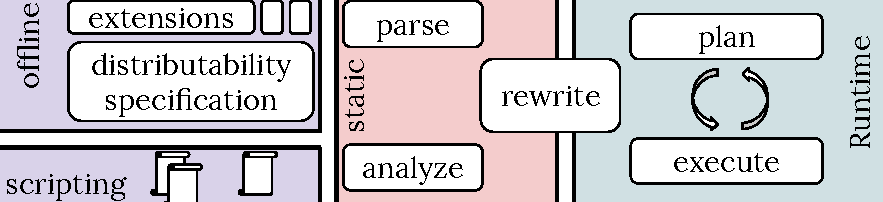
\includegraphics[width=0.49\textwidth]{\detokenize{./figs/dish_overview.pdf}}
\caption{
  \textbf{High-level schematic.}
  \sys leverages distributability analysis for built-in commands and any developer extensions (left) to automatically transform shell scripts (mid) and orchestrates their
  execution (right).
}
\vspace{-15pt}
\label{fig:schematic}
\end{figure}


Unfortunately, developing $p_1$'s distributed equivalent requires a significant effort.
% For a user with many computers and larger inputs, 
% The scope of such rewrites, and therefore the cost of manual effort, can vary considerably.
For simple pipelines, fitting into restricted models of computation, this effort amounts to expressing the computation using the primitives provided by a big-data framework~\cite{mapreduce:08, ciel:11, spark:12, naiad:13} or domain-specific language~\cite{alvaro2011consistency, distal:13, meiklejohn2015lasp}---an unjustifiable cost for one-off pipelines that take a few minutes to compose (but are applied to large datasets).
More complex pipelines, such as the ones presented in later sections, would involve a full-fledged distributed programming language~\cite{erlang:96, lopes1997d, acute:05, mace:07, cloudhaskell:11, ScalaLoci:18}. %  or a distributed operating system---\eg Plan9's \ttt{rc} shell.
In both cases, manual rewriting is expensive and can introduce new bugs, cascading changes, and divergence from legacy functionality.
Could the generation and execution of $p_1$'s distributed version be fully and correctly automated?

To answer this question, this paper presents \sys, a shell \todo{preprocessor} that transforms shell pipelines into their distributed equivalents, enabling \emph{distribution-oblivious programming}.
The key insight behind \sys is that the language of the Unix shell already encodes stream processing, providing most of the information required to distribute a computation
% FIXME \kk{I am not sure whether stream processing provides information for distributing a computation on its own. Maybe we can say that the shell exposes operator level parallelism, and that this is the first step to distributing a computation}.
\sys builds on this insight with a careful study of the distributability properties of shell primitives and commands, a pipeline rewriting pass that identifies \todo{maximal} sub-expressions as candidates for scale-out, and a late-bound command-prefixing scheme for deferring scheduling decisions to the distributed planner (\ie when runtime information is available).
A \sys-enabled $p_1$ will run \ttt{tr}s in parallel streams,
  use a mostly-parallel tree of \ttt{sort}s,
  run \ttt{uniq} mostly in parallel,
  \ttt{head} in one of the streams,
  and (trivially) merge streams in \ttt{out}.

The combination of automated transformations for program distribution with the ability to maintain correct non-distributed semantics results in several benefits.
% \sys converts legacy shell pipelines into their distributed equivalents fully automatically, offering $100\times$ improvements in performance without a single line of additional code or annotation.
First, shell users composing pipelines (or simply running legacy pipelines on massive datasets) can see scalability benefits without any manual effort---no need for \ttt{qsub}~\cite{gentzsch2001sun}, \textsc{SLURM}~\cite{yoo2003slurm}, calls to \textsc{GNU} \ttt{parallel}~\cite{Tange2011a}, or any manual rewriting~\cite{mapreduce:08, ciel:11, spark:12}.
Second, developers of new shell commands can use a concise a domain-specific language to express their distributability properties rather than using ad-hoc, command-specific flags such as {\tt -t},  {\tt NUM\_THREADS}, \ttt{-t}, \ttt{-p} \etc
Most importantly, \sys provides an architectural lesson for system designers---namely, that large-scale research efforts in the distributed- and operating-system literature to provide a \unix-like distributed equivalent~\cite{ousterhout1988sprite, mullender1990amoeba, pike1990plan9, barak1998mosix} would have been simplified by a thin (but sophisticated) rewriting shim like the one \sys provides.
% Nice critique on parallel: https://bugs.debian.org/cgi-bin/bugreport.cgi?bug=597050#75

% % Make Unix benefits explicit?
% Indeed, the primary reason behind $p_1$'s succinctness is that the pipeline is a domain-specific language for describing operations over streams.
% Key elements of \unix are the ability to compose programs written in different languages, the abstraction of a file system as a set of resident streams, a small but extensible library of commands, and the ability to resolve names within a global context.
% Under the hood, the \unix kernel buffers results, synchronizes processing stages, and generally orchestrates the computation.

The paper is structured as follows.
It first starts with a background section outlining pipeline concepts and overviewing \sys~\sx{bg}.
Sections \ref{distributability}--\ref{recipes} highlight key contributions:
\begin{itemize}

  \item
  \S\ref{distributability} overviews \sys and introduces several scalability and distributability classes.

  \item
  \S\ref{ir} presents a set of rewriting transformations for identifying maximal pipeline sub-expressions, candidates for scale-out.

  \item
  \S\ref{impl} details other concerns, such as distributed state management and extensibility.
\end{itemize}

\noindent
\sys's evaluation~\sx{eval} shows significant speedups on both parallel and distributed execution, using a combination of micro-bench\-marks---popular shell one-liners that highlight certain features---and multi-line macro-benchmarks---a web crawling and indexing engine, a genomics pipeline, and a popular weather analysis script.
After a comparison with related prior work~\sx{related}, the paper closes with a discussion of related work and possible future directions~\sx{discussion}.
% \bigskip
% \begin{quote}
% \footnotesize
Additional material, in anonymized form, is available at
\href{https://git.io/Je6Nk}{https://git.io/Je6Nk}.
% \end{quote}

% \begin{figure*}[t]
% \centering
% 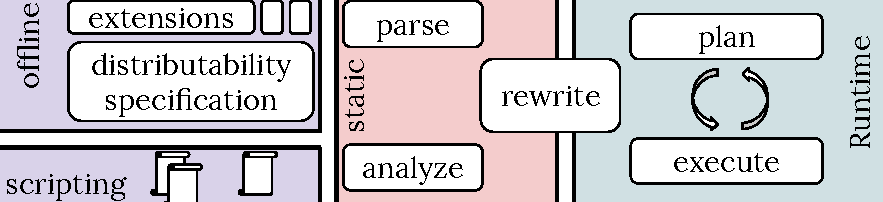
\includegraphics[width=0.49\textwidth]{\detokenize{./figs/dish_overview.pdf}}
% \caption{
%   \textbf{Applying \sys to $p_1$.}
% }
% \label{fig:example}
% \end{figure*}
% 

\section{Background and Overview}
\label{bg}

This section presents (i) important background on shell pipeline composition~\sx{bg:pipelines}, and (ii)) a high-level overview of \sys's design and implementation.

\subsection{Unix Composition, Informally}
\label{bg:pipelines}

% A pipeline is a mechanism for program composition that works by chaining together programs (or, \emph{commands}) using pipes.
\unix provides several ways for succinct program composition.
Central among them is the \emph{pipe}, a primitive that passes the output of one program as input to the next.
These programs produce output and consume input concurrently, and possibly at different rates, with the \unix kernel facilitating program scheduling and communication synchronization behind the scenes.
Intermediate programs, termed commands, can also be developed in different programming languages, as long as they conform to a common interface.
%\begin{wrapfigure}{r}{0.06\textwidth}
%  \vspace{-12pt}
%  % \begin{center}
%    % \includegraphics[width=0.48\textwidth]{gull}
%    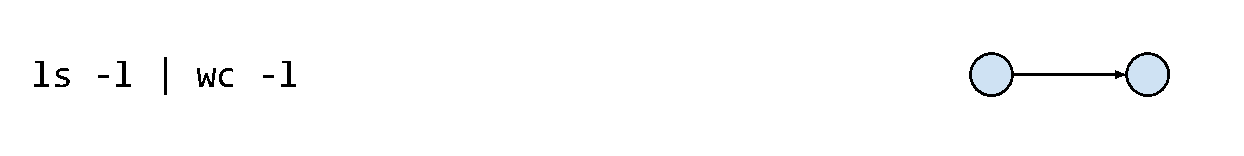
\includegraphics[width=0.06\textwidth]{\detokenize{./figs/dish_ex1.pdf}}
%  % \end{center}
%  \vspace{-30pt}
%\end{wrapfigure}
This interface exposes a stream of contiguous character lines.
A few characters are special---for example, the newline (\textsc{NL}) character delineates an element of the stream, and the end-of-file (\textsc{EOF}) character signals the end of a stream.
As part of this interface, each command has access to (any combination of) three \emph{standard} streams---input, output, and error.
% the input stream (stdin), the output stream (stdout), and the generating errors or diagnostics to the standard error stream (stderr)
% generating errors or diagnostics to the standard 
% Leveraging this interface, pipelines chain together commands by their standard streams, such that the output stream of one command (stdout) is passed directly as input (stdin) to the next one.
\smallskip
\begin{lstlisting}[language=sh, numbers=none, escapeinside={($}{$)}]
  ls -l | wc -l                          [($$p_2$$)]
\end{lstlisting}
\smallskip
Commands can be tuned by two mechanisms, namely com\-mand-line options and environment variables.
Options control the execution of a program---\eg changing the \ttt{sort}ing order.
The shell does not have any visibility into these options; 
  after it expands special characters such as \ttt{~} and \ttt{*}, it leaves parsing and evaluation entirely up to every command.
Environment variables carry more general information about the surrounding system---\eg file search paths, system defaults, parsing switches \etc 
They are organized in a map from names to values, both of which are strings, and can be evaluated at any point in the program---including as commands, flags, a shell feature termed parameter \emph{expansion}.

% TODO: Talk about security primitives?
Streams are a key feature of \unix, and go hand-in-hand with the file abstraction:
  files are simply persistent streams that can be manipulated by commands or pipelines.
% \begin{wrapfigure}{r}{0.15\textwidth}
%   \vspace{-15pt}
%   % \begin{center}
%     % \includegraphics[width=0.48\textwidth]{gull}
%     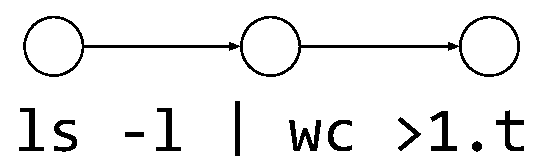
\includegraphics[width=0.15\textwidth]{\detokenize{./figs/dish_ex3.pdf}}
%   % \end{center}
%   \vspace{-25pt}
% \end{wrapfigure}
Reading a file or a set of files generates a stream; 
  similarly, streams can be trivially redirected to the file system---by appending with the file identifier.
Files are named, in the sense that they correspond to a global identifier---for example, \ttt{/x/y} corresponds to a persistent stream.
\unix exposes a few different types of files---\eg directories, symbolic links, named pipes (or FIFOs), and special character devices.
As a result, file-system identifiers part of a pipeline may resolve to in-memory structures or pseudo-devices (\eg \ttt{/dev/urandom}).

% At a high level, POSIX defines several file types:
% (-) regular files, storing lines of text or binary data,
% (d) directories, grouping together multiple other files,
% (l) symbolic links, pointing to other files,
% (p) named pipes or FIFOs, communication primitives that can be named and manipulated like files,
% (s) domain sockets or DSes, full-duplex communication primitives that support passing file descriptors, and
% (b or c) special files, interfaces to device drivers or low-level abstractions, presented as ordinary files.
\smallskip
\begin{lstlisting}[language=sh, numbers=none, escapeinside={($}{$)}]
  ls | sed 's/1/2/' | > out.t 2> err.t    [($$p_3$$)]
\end{lstlisting}
\smallskip

\noindent
Special files are particularly interesting because they are resolved to OS structures.
One example is the special \ttt{/proc} filesystem (procfs) that presents information about processes and the operating system, offering a feature analogous to programmatic introspection:
  with \ttt{procfs} commands can inspect and alter their directory or the flags passed to them.
% Here are a few examples:
% (i) \ttt{/proc/PID/cmdline} contains the command that originally started the process,
% (ii) \ttt{/proc/modules} contains a list of the kernel modules currently loaded, and
% (iii) \ttt{/proc/PID/cwd} contains a symlink to the current working directory of the process.
Similarly, \unix exposes file-system handles for various ephemeral structures, including standard streams.
This bidirectional relationship between ephemeral streams and persistent names---the fact that streams can be named in the file-system and files can be converted to streams---is a key enabler of the runtime rebinding achieved during our transformations.

A small but powerful set of features is concerned with stream manipulation.
Some of these features are built into the shell;
  for example, given a file identifier, stream redirection operators can direct stdout or stderr to a file.
% \begin{wrapfigure}{r}{0.15\textwidth}
%   \vspace{-15pt}
%   % \begin{center}
%     % \includegraphics[width=0.48\textwidth]{gull}
%     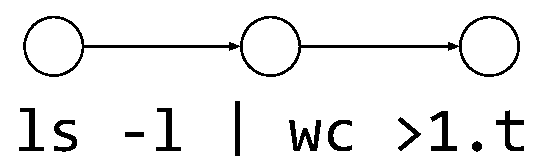
\includegraphics[width=0.15\textwidth]{\detokenize{./figs/dish_ex3.pdf}}
%   % \end{center}
%   \vspace{-25pt}
% \end{wrapfigure}
As described before, the file can be a FIFO dubbing as input to another command.
More interestingly, some commands allow splitting (resp. merging) a single stream (resp. many streams) into multiple streams (resp. a single stream);
  stream merging can be achieved by appending one stream after the end of another or by fusing (zipping) streams column-wise into a single (fat) stream.
% TODO: talk about \ttt{xargs}?

\smallskip
\begin{lstlisting}[language=sh, numbers=none, escapeinside={($}{$)}]
  cat * | tee >(wc -l > l.t) | zip > a.z   [($$p_4$$)]
\end{lstlisting}
\smallskip

\noindent
% Explicit Redirection, Implicit splitting and merging, This can be done through the file-system operators 
The combination of ephemeral file-system identifiers and the stream redirection described above enable surprisingly expressive pipelines. %---for example:
The most interesting feature of these pipelines is the presence of cycles:
  a pipeline segment processes some input, part of which is extracting the next input to process.
One example use case, discussed in the evaluation section~\sx{eval} is a web crawler that feeds extracted URLs from the input stream back to the start of the pipeline.
% These streams are created by the C library (glibc) at the start of program execution,
% and new streams can be created to connect to files, sockets, pipes,

\smallskip
\begin{lstlisting}[language=sh, numbers=none, escapeinside={($}{$)}]
  read | { calc | square; } >/dev/fd/0     [($$p_5$$)]
\end{lstlisting}
\smallskip

\noindent
Apart from pipes, the \unix shell provides several other forms of program composition such as sequential (\ttt{;}) and parallel (\ttt{\&}) composition operators.
Command substitution, expressed as \ttt{\$($c$)}, replaces the expression with the results of executing $c$.
Code blocks, expressed as \ttt{\{$c_1; c_2$\}}, can redirect streams for the entire group of $c_1$ and $c_2$;
  this is analogous to an anonymous function, which contains many statements and can possibly be assigned to a variable that can later be invoked with parameters.
Subshells, enclosed in \ttt{($c_1; c_2$)}, are similar to code blocks but spawn a child shell, thus avoiding the pollution of their environment variable context. % but incurring higher overhead.

\unix pipelines are surprisingly powerful, a feature that \sys exploits by re-targeting shell scripts during its rewriting passes that target shell.

% \begin{lstlisting}[
%   language=es,
%   mathescape,
%   float=t,
%   belowskip=-5mm,
%   label=core-pl,
%   upquote=true,
%   caption={
%     \textbf{The core language of the POSIX shell.}
%     The language used by ; file identifiers and expansion are not shown.
%   }]
% $p$ ::= $s\in{}String$ | $n\in{}Number$ | $b\in{}Bool$ | $\emptyset$
% $v$ ::= $p$ | ($x$,$\ldots$) => {e} | {$s$:$v$,$\ldots$} | [$v$,$\ldots$]
% $e$ ::= x | $v$ | ($x$ = $e$) $e$ | $e$($e$) | $e$[$e$] = $e$
% \end{lstlisting}

% \begin{lstlisting}[language=sh, float=h, numbers=none, escapeinside={($}{$)}]
%  cat /proc/ >                            (($$p_4$$))
% \end{lstlisting}
% \begin{lstlisting}[language=sh, float=h, numbers=none, escapeinside={($}{$)}]
%  cat /proc/ >                            (($$p_5$$))
% \end{lstlisting}
% \begin{lstlisting}[language=sh, float=h, numbers=none, escapeinside={($}{$)}]
% { echo 1; echo 2; } > out.txt
% \end{lstlisting}

\begin{figure}[t]
\centering
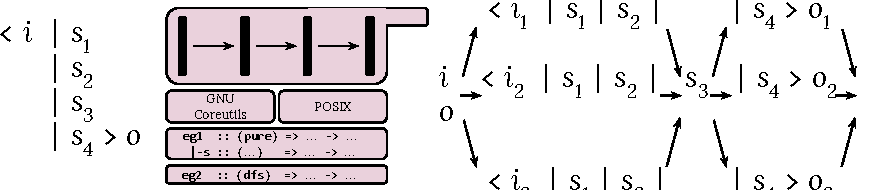
\includegraphics[width=0.49\textwidth]{\detokenize{./figs/dish_schematic.pdf}}
\caption{
  \textbf{\sys transformation overview.}
  Given a shell pipeline, \sys leverages command distributability to identify
  high-distributability stages, rewrite them, and orchestrate their execution.
}
\vspace{-15pt}
\label{fig:overview}
\end{figure}


% \heading{Generation}
% Expansion---the key is that expansion and evaluation are handled by the shell at an earlier stage 
% The most powerful---and interesting, for \ttt{dish}---type of expansion is subshell expansion, that allows replacing entire input streams 

\subsection{\sys Design Overview}

As outlined earlier, the key insight behind \sys is that the shell already describes parallel computations over streams.
Intuitively,
 (i) the parallel-composition operator exposes \todo{task} parallelism
% FIXME \kk{I have named that operator level parallelism, which one do we prefer?},
 (ii) commands such as \ttt{xargs} and \ttt{tee} expose data parallelism,
 (iii) the pipe operator is candidate for both task and data parallelism, and
% \kk{How does it enable data parallelism?} \nv{added "candidate", helps?}
 (iv)  other composition operators can be viewed as barrier candidates.
To leverage these insights and correctly distribute a pipeline such as $p_1$, \sys must solve several challenges.

% However, understanding the shell's primitives is not enough
\sys needs to understand the distribution characteristics of individual commands used to compose larger programs~\sx{distributability}.
This challenge can be broken down into two parts.
First, there is a need to understand the commands already in the shell---that is, built-ins that come with any shell and support its core functions.
One example is the set of commands defined by the \textsc{POSIX} standard~\cite{}.
\sys addresses this part by a careful study of a group of commands, identifying a small but clear set of well-understood distributability classes.
This set is already useful enough to allow the composition of practical pipelines~\sx{eval}.

The second part is expressing such characteristics extensions that fall outside the built-in set, allowing new commands to leverage \sys's power.
Commands are arbitrary programs, but still conform to the shell's pipeline interface.
To solve this part, \sys leverages the prior study to define a small but expressive domain-specific language (DSL) for describing a command's key properties with respect to its distributability.
Using this DSL, developers of commands (not users of the shell) can quickly and easily capture the class of the command.
A command developer can only annotate the default behavior;
  if a new flag is added a few years later, and if that flag alters the command's class, only then a new annotation is needed.

Given a set of commands composed together by the shell primitives, \sys's next challenge is to analyze it and identify candidate subexpressions for distribution~\sx{ir}.
\sys addresses this challenge with a series of rewriting passes that perform dataflow analysis for identifying \todo{maximal} distributable sub-expressions.
It converts the AST to a dataflow graph, and iteratively performs graph transformations that expose data parallelism as task parallelism while preserving correctness.
These transformations are complicated by the shell's pervasive use of dynamic features---\eg environment variables, file input sizes, \etc

Finally, \sys needs to schedule and execute the distributed dataflow graph.
To achieve this, \sys's runtime component needs to solve several challenges~\sx{impl}.
First, \sys needs to wrap single-node commands with corrective runtime interposition based on their classes;
  this is achieved by thin wrappers for all the commands involved in the program, generated just-in-time using the distributability specification outlined earlier.
The reasoning behind wrappers being thin is to not interfere with legacy functionality---commands have many flags accumulated over long periods of time.

Second, \sys needs to fill-in planing details left blank by the rewriting pass.
This is achieved with \emph{planner activators}, commands that yield (and pass their arguments) to the scheduler.
From the point of view of the shell, planner activators are expressed through a higher-order command---similar to \ttt{xargs} and \ttt{time}---that takes other commands as arguments.
Planner activators achieves the latest possible binding, when critical runtime information is available.
% FIXME \kk{I am not exactly sure I understand that :) } \nv{which part?}

The next few sections discuss \sys's design and implementation details.
They also outline other, less obvious challenges---such as the synchronization of environment variables, distributed file operation, \etc.


\section{Distributability Classes}
\label{distributability}

To have any hope of distributing \unix pipelines, \sys first needs to understand the distribution characteristics of their intermediate commands.
This understanding is encoded in a command's \emph{distributability} class.
Informally, a distributability class represents the level of synchronization required by copies of a command executing in parallel.
It focuses on characteristics that are important for distribution, rather than all the observable behavior of a command.
\sys leans towards a few coarse classes rather than many detailed ones---among other reasons, to simplify their use by command developers.
% Make the connections that this is like a type, that doesn't capture everything, but is good-enough

This section starts by defining these classes, paired with a distributability study of the commands found in standard libraries such as {\sc POSIX} and GNU Coreutils~\sx{cmd}.
Building on this study, it presents a DSL that enables command classification by its developers~\sx{ext}.
In return, \sys uses this DSL to tag commands in the standard libraries and generate their wrappers, as presented in later sections.

\subsection{Distributability of Standard Libraries}
\label{cmd}

% nv TODO: this is a hierarchy
Broadly, shell commands can be split into five major classes (summarized in Tab.~\ref{tab:classes}) with respect to their distribution characteristics, depending on how they interact with state.
These classes are ordered in ascending difficulty of distribution:
  later classes require more effort.
In this order, each class can be thought as a subset \kk{I am not sure this holds for all classes. I would propose saying that some classes are subsets, e.g....} of the next one---\eg all stateless commands are pure---meaning that the synchronization mechanisms required for any superclass would work with its subclass (without seeing any performance improvements).

\begin{table}[t]
\center
\footnotesize
\setlength\tabcolsep{3pt}
\caption{
  \footnotesize{
    \textbf{Distributability Classes}.
    Broadly, \unix commands can be broken down into to five classes.
  }
}
\begin{tabular}{l @{\extracolsep{\fill}} lll}
\toprule
Class                           &  Key    & Example Commands                            & Coreutils       \\ % & POSIX       \\
\midrule
Stateless                       & ~\tsta  & \tti{tr},   \tti{cat},    \tti{grep}        &  22 (21.1\%)    \\ %  &           \\  % 22
Pure                            & ~\tpur  & \tti{sort}, \tti{wc},     \tti{uniq}        &  21 (20.1\%)    \\ %  &           \\  % 21
(Distr.) File-System~           & ~\tdfs  & \tti{cp},   \tti{ln},     \tti{rm}          &  27 (25.9\%)    \\ %  &           \\  % 27
Side-effectful                  & ~\tsid  & \tti{env},  \tti{chroot}, \tti{whoami}      &  25 (24\%)      \\ %  &           \\  % 25
Irreversible                    & ~\tirr  & \tti{exit}, \tti{lpr},    \tti{reboot}      &  5  (0.4\%)     \\ %  &           \\  % 5
% \midrule
% Shell PL Constructs             &                         &                  \\
% \etc                            &                         &                  \\
\bottomrule
\end{tabular}
\label{tab:classes}
\end{table}


% \heading{Preliminaries}
% \heading{POSIX, GNU Core-utils, and beyond}

\heading{Stateless Commands}
The first class contains stateless commands~\sta that operate on individual elements of the stream, without maintaining state across invocations.
These are commands that can be expressed as a purely functional map---\eg \ttt{basename} removes a path prefix from a string and \ttt{grep} filters out individual lines.
At times, stateless commands may operate as functions that produce multiple elements---\eg when they insert a {\sc NL} token.
Workloads that use only stateless commands are trivial to parallelize:
  they do not require any synchronization to maintain correctness, nor caution about where to split.
 % map :: (a -> b) -> [a] -> [b]

Many of these commands (about 1/3 of coreutils' \sta) are stateless \emph{within} an element (\eg \ttt{tr} transliterates characters, one at a time).
This property could allow further parallelization within a single line element, a feature that might seem of limited use because these commands are not particularly expensive computationally precisely due to their narrow focus.
However, it is useful for cases with very large stream elements (long lines) such the \ttt{.fastq} format used in bioinformatics pipelines.

\heading{Pure Commands}
The second class contains pure commands \pur.
These commands respect functional purity, returning the same results for the same inputs, but maintain internal state across their entire pass.
The details of this state and its propagation during piecewise element processing affects their distributability characteristics.

Some commands are easy to parallelize, because they maintain trivial state and are commutative---\eg \ttt{wc}, which simply maintains a counter.
Others, such as \ttt{sha1sum}, maintain more complex state that has to be updated in a sequential fashion.

Often these commands do not operate in an online fashion, but need to block until the end of a stream---a typical example of this is \ttt{sort}, which cannot start before the last line of input has been consumed.
Non-streaming constraints affect task parallelism, but not data parallelism:
  \ttt{sort} can be parallelized significantly using divide-and-conquer techniques, that is implementing it as a map and a reduce function.

\heading{File-system Commands}
The third class contains commands that access the file-system~\dfs.
This is the largest class, as the file (and file-system) abstraction is central to the \unix design and philosophy~\cite{unix}.
In fact, \unix uses the file-system as a proxy to several file-unrelated operations---\eg access control and device driving is grafted upon the file-system.

% TODO: mention that some commands fail to comply with the interface---for example, csplit could be split followed by a redirection to files.
Commands in \dfs are distributable for many reasons, as evidenced by a long history of distributed \unix file-system clones~\cite{catalogue}.
Some of these offer the semantics of the \unix file-system---hierarchies, protection bits---and a POSIX virtualization layer that enables support for the commands in \dfs.
The vast majority of these commands are control-plane operations that act on identifiers~\sx{bg}---for example, \ttt{touch} for creating a file or \ttt{chgrp} for changing group ownership.
% these operate by changing an inode
Data-plane operations on files go explicitly through stream-redirection operations~\sx{bg}.
Operations using different identifiers pose no problems;
  operations sharing a single identifier might have problems---but these risks exist even in the non-distributed case.
While such pathological cases are possible, they are rare enough---and have been rare enough since \unix's inception~\cite[\S3.6]{unix}).

% \unix itself does not offer any guarantees when a file is accessed concurrently on a single computer.

\heading{Side-effectful Commands}
Another large class of commands are ones that have side-effects to memory~\sid.
Because of timesharing and multi-tasking---\ie the fact that many users can operate multiple terminals on single \unix machine---a subset of these commands are devoted to accessing and sharing memory such as environment variables and shell parsing flags.

A command in \sid will require some form of concurrency control to distribute property.
However, because its side-effects stay within the distributed \unix environment, they can be manipulated using---including optimistic and multi-versioning schemes that can roll-back side-effects.

The vast majority of these commands (a ratio of 21:4) only \emph{read} values, and usually values that are never affected by the user.
For example, \ttt{date}, \ttt{uname}, and \ttt{finger} are all commands that interface with kernel- or hardware-generated information that is not writable by user-space scripts.
Even if \sid commands are protected with transactions
  these benefits are even greater for read-only or read-mostly accesses.

\heading{Irreversibly Side-effectful Commands}
Finally, some commands have side-effects outside \sys---for example, by printing a file with \ttt{lpr} or restarting with \ttt{reboot}.
Such commands are not distributable---they have to refer to a single location---and have to be guarded with pessimistic transaction control mechanism.

\heading{Discussion}
There are several technical details about \sys's design decisions worth noting.

In terms of inputs, \sys supports commands with multiple input (resp. output) streams, by prepending (resp. appending) shell built-ins that merge input (resp. split output) streams~\sx{impl}.
Thus, a command can be modelled as having one input and one output stream, a representation that is used throughout \sys including the extensibility DSL~\sx{ext}.

Wanting to present the full picture for completeness purposes, the focus for the rest paper will be commands in \sta and \pur.
Other commands are treated as  non-distributable for now~\sx{conclusion};
  by building infrastructure to handle other classes, \sys would be able to (i) extract more parallelism and (ii) handle larger programs.
Even with only these two classes, however, \sys supports highly useful pipelines that are more expressive than ones in popular frameworks such as Hadoop~\cite{mapreduce:08} and Spark~\cite{spark:12}~\sx{eval}.

\subsection{Extensibility}
\label{ext}

%% Here is the type for \ttt{bwa}, a command that performs a Burrows-Wheeler transform over genomic data:
%% % ( bwa ) :: ( Pure )  => { In \/ File* } -> { Out /\ Err }    -- default case
%% %    | -h :: ( Sless ) => { Out }                              -- if needed
%% \begin{lstlisting}[language=sh, float=h, numbers=none, escapeinside={($}{$)}]
%% (bwa) :: (Pure) ($$\Rightarrow$$){In($$\lor$$)File*}($$\rightarrow$$){Out($$\land$$)Err}
%%   |-h :: (Sless)($$\Rightarrow$$){Out}                              
%% \end{lstlisting}

%% It states that the command defaults to the Pure class.
%% It's operation can be thought as a transformation from input streams to output streams.
%% It operates either on stdin or, if this doesn't exist, one or more files specified as arguments;
%% % TODO: check actual man page for how to specify files
%%   it writes to the output and error stream rather than a file.
%% The \ttt{-h} flag moves \ttt{bwa} into the Stateless class;
%%   its output is a constant function.

% FIXME: \nv{TODO: remember to bubble up(me)}
An important characteristic of the \unix shell is its language-agnostic extensibility~\sx{bg}.
Users composing pipelines are free to install custom commands available from various sources.
Being general programs, commands are developed in a variety of languages and are extended over long periods of time.
%% \kk{Text point: This restricts the space of solutions for
%%   distribution of shell scripts}
As a result, any static characterization of shell commands is unsatisfactory as it would quickly become obsolete, supporting only a small subset of commands.
This poses a challenge to the developers of individual commands---how can they augment their commands to capture information critical to \sys without too much effort?
%% \kk{Text point: The characteristics of a good solution}

To address additions and changes to the set of commands available to the shell, \sys provides command developers a lightweight, domain-specific language (DSL).
The DSL allows developers to express semantic information about a command's distributanility that is critical to \sys.
This DSL can be used by the developers of new commands to succinctly express this information, such the class of a command and the sequence of sources from which it reads its input.
It could also be used by developers that extend or maintain existing commands, to express additions or changes to the command's implementation or interface.

\heading{Command-line Options}
As described earlier~\sx{bg}, command-line options and environment variables can affect the operation of a command.
Options are a particularly popular way to control a command, 
  directly affecting a command's distributability classification.
That is, commands are assigned to default classes, and options can change the class in which they belong.

As simple examples, consider \ttt{cat} and \ttt{sort}.
By default \ttt{cat} is in \sta, but with \ttt{-n} it jumps into \pur because it has to keep track of a counter.
Conversely, \ttt{sort} defaults to \pur, but \ttt{with} \ttt{-h} it jumps into \sta.
% TODO: closure?

%% Can be tweaked according to this:
%% https://tex.stackexchange.com/questions/24886/which-package-can-be-used-to-write-bnf-grammars

\begin{figure}
  \centering
  \begin{grammar}
    <option> ::= `-' <string>

    <category> ::= `stateless' | `pure' | ...

    <maybe-int> ::= | <int>

    <arg> ::= `args[' <int> `]'

    <args> ::= <arg>
    \alt `args[' <maybe-int> `:' <maybe-int> `]'

    <input> ::= `stdin' | <args>

    <inputs> ::= <input>
    \alt <input> `,' <inputs>

    <output> ::= `stdout' | <arg>

    <option-pred> ::= <option>
    \alt `value' <option> = <string>
    \alt `not' <option-pred>
    \alt <option-pred> `or' <option-pred>
    \alt <option-pred> `and' <option-pred>

    <assignment> ::= `(' <category>, `[' <inputs> `]' , <output> `)'

    <predicate> ::= <option-pred> `=>' <assignment>

    <pred-list> ::= `|' <predicate> <pred-list>
    \alt `|' `otherwise' `=>' <assignment>

    <command> ::= <name> `\{' <pred-list> `\}'

    <command-list> ::= <command>
    \alt <command> <command-list>
  \end{grammar}
  \caption{
\textbf{Distributability description language.}
The DSL captures important information regarding the distributability of a command.
\vspace{-20pt}
}

  \label{fig:dsl}
\end{figure}



\heading{Command Inputs and Outputs}
%
Consider the command \ttt{comm}. It takes as input two files and
performs a join operation. When invoked without any option, it
produces three-column output. The first column contains lines that
unique to the first file, the second column contains lines that are
unique to the second file, and the last column contains lines that
exist in both files. In the general case \ttt{comm} is in \pur, since
it needs to wait until it reads both files completely before it can
output its results.

However, \ttt{comm} can also be invoked using some options that
suppress the output of any combination of columns. More precisely, the
option \ttt{-1} suppresses the first column of the output. Similarly,
\ttt{-2} and \ttt{-3} supress the second and third column. Using both
\ttt{-2} (or \ttt{-1}) and \ttt{-3}, the command becomes \sta
regarding its first (resp. the second) file argument.

% \ttt{comm} is in \pur, but with \ttt{/input1} it jumps into \sta---as it is now partially evaluated, it becomes stateless with respect to the second argument.

\heading{Distributability DSL}
%
\sys's distributability description DSL (Fig.~\ref{fig:dsl}) is
designed to be able to classify a commands into multiple categories
given their options.

It assumes that the arguments of a command can always be separated to
options and file arguments (checking if they start with a
\ttt{-}~\footnote{Note that the single character \ttt{-} is not an
  option as it is most often used to designate that a command reads
  from its standard input}). A file written in the language contains a
record containing a mapping from predicates to assignments for each
command. Predicates can be simple boolean formulas on the existence
and the value of any option. Each assignment contains the command
category, the sequence of its input sources, and its output
source. Inputs to commands are a sequence of file arguments and its
standard input. Similarly, the output is either its standard output or
a file argument. An example record for comm can be seen below:

\begin{lstlisting}[float=h, numbers=none]
  comm {
    | -1 and -3 =>
      (stateless, [args[1]], stdout)
    | -2 and -3 =>
      (stateless, [args[0]], stdout)
    | otherwise =>
      (pure, [args[0]], stdout)
  }
\end{lstlisting}

The semantics of the language is straightforward: given a command, the
interpreter collects its options and then returns the assignment of
the first predicate that is satisfied. The final predicate is always
satisfied. For example the following two invocations of \ttt{comm}
would be classified as follows:

\begin{lstlisting}[language=sh, float=h, numbers=none, escapeinside={($}{$)}]
 comm -13 f1 f2 # => (stateless, f2, stdout)
 comm f1 f2     # => (pure, f1, stdout)
\end{lstlisting}



\tr{We don't need to designate the stderror, because we assume that it
  is never the main output of a command and it will never be used by
  the input of another command in the pipeline. If someone indeed
  wants to do this, they can just use a redirect I think to get around
  it.}


\tr{If we talk about the language it would be good to give some
  statistics about how many commands (out of the ones that we have
  classified) can be represented with one, two clauses etc. If we have
  a different solution (like python function that given a command and
  its arguments returns the category) then we could talk about how
  many lines of code it took to categorize all the commands that we
  did.}


\tr{Note: Since a categorization language will probably not be
  complete (especially the one showing the input arguments) there
  should be a backup mechanism, when the language is not expressive
  enough, like a python function that categorizes the command, and
  returns its input argument if it is stateless.}

\tr{(Maybe) We should have a crisp point about why we have this categorization
  language, and why don't we just allow someone to write a function in
  python for each command, that given the command and its arguments,
  returns whether the command category. Possible arguments include,
  the fact that this language is simpler to use, especially by non
  experts that just run some script but have installed some commands
  that are not ``supported''. Another possible argument is that we
  could be able to reason about the constructs of the categorization
  lagnauge, and that they will be easier to read and
  understand. Another argument is that since these categorizations
  should be shareable among users, it would be bad to execute
  arbitrary python code, so using this language, expressivity is
  limited. All of these arguments are a little bit weak though. Niko,
  what do you think?}


\heading{Pure Commands}
%
Together with the commands in \sta, that are always easy to
parallelize, there also exists a subclass of commands in \pur that can
be parallelized by separating them into a map and a reduce
operation. In order to allow command developers to extend \sys with
information about how to parallelize new pure commands, \sys offers an
interface to specify how to distribute a pure command.

\TODO{I am not sure a general interface is so easy to design. It needs
  more though. It might be beneficial to just talk about sort and wc
  here and how we implemented them and nothing more. Or maybe this
  could then go to the implementation? Or maybe say that one can write
  a python function that given a node of the graph, transforms it into
  many. I am not sure what is best...}


% As mentioned in distributability, pure commands can be broken down
% into different categories. We might be able to get ideas about this
% from this paper:
% \url{http://www.cs.toronto.edu/~azadeh/papers/pldi17-ex.pdf} and its
% continuation in PLDI 2019.
% FIXME: \nv{Cite this paper?}
\tr{Can we find a solution for the commands in coreutils?}


\section{Dataflow Graph Model}
\label{ir}

In order to effectively apply optimizations and distribute a shell
script, it first has to be translated to a manipulable
representation. As mentioned in \Cref{bg:pipelines}, the two main
abstractions of the shell, are files that contain data, and commands
that communicate through these files. We propose a slight variation of
the standard dataflow graph model, that is commonly found in stream
processing systems, as the representation of a distributed shell
computation. The main benefit of the dataflow graph model is that it
clearly exposes task parallelism, as different nodes can be
independent processing workers. In our case each node represents a
command, and each edge represents a file.

\subsection{Graph Components}

\paragraph{Nodes - Commands}

For a set $D$, we write $D\kstar$ to denote the set of all finite
words over $D$. For words $x, y \in D\kstar$, we write $x \cdot y$
or $xy$ to denote their concatenation. We write $\eps$ for the empty
word. We say that $x$ is a \emph{prefix} of $y$, and we write $x \leq y$, if there is a word $z$ such that $y = xz$. It is easy to see that $\leq$ is a partial order, and it is often referred to as the \emph{prefix order}.

A node $f$ of the graph represents a function from one (possibly empty)
input stream to an output stream $f : D\kstar \to D\kstar$, where $D$
represents the basic data type of a line of characters. This
representation captures the majority of shell commands. We require that
the function $f$ is monotone w.r.t.\ the prefix order. This captures
the idea that a node cannot retract output after it has been emitted.
%More formally, $\forall f, x, y, f(x) = y$, then for any $x'$, there exists $y'$ such that $f(x.x') = y.y'$, where $.$ is standard
%concatenation and will be omitted when obvious.
An example of a node is the following command:

\begin{lstlisting}[language=sh, float=h, numbers=none, escapeinside={($}{$)}]
 grep ``foo''
\end{lstlisting}

\noindent
This command takes a stream of lines from its standard input and
returns a stream of lines on its standard output. An important
observation is that commands in the shell might read their input
stream from a sequence of different sources. An illustrative example
is the command \ttt{cat} which reads its input from a combination
of files and its standard input.

\begin{lstlisting}[language=sh, float=h, numbers=none, escapeinside={($}{$)}]
 cat x - y
\end{lstlisting}

The example above reads file \ttt{x} until it encounters the EOF
character, then reads from \ttt{stdin}, and then reads from
\ttt{y}. In order to handle this particularity, nodes in the
dataflow graph can have many incoming edges, that are ordered in a
sequence. Note that this does not correspond to standard dataflow
graph representations where the semantics of multiple incoming edges
is either zipping the inputs in pairs, or arbitraliy interleaving them.

\TODO{Is the following paragraph best suited here? It describes an
  assumption that we make about commands, to guarantee the validity of
  our transformations. The assumption is needed due to the limitation
  of the programming model of one input one output per command.}

Note that nodes can read from more files than just the files of their
stream (or respectively write to more files that their output stream),
however these files are static (e.g. used for configuration or logging
\kk{Would an example here help}) and do not represent streams of data,
and therefore are not considered part of the dataflow graph. We assume
that these static files can only be accessed by one node, thus
ensuring that they do not interfere with the distributed
implementation.
%% Because of the assumption in section Front End \ref{}, that each file
%% exists only once in the dataflow graph, we can safely assume that
%% reading and writing to these static files does not interfere with the
%% distributed implementation, and doesn't alter the behaviour of the
%% program.

\paragraph{Edges - Files}

Edges in the dataflow graph represent files, the basic data
abstraction of the shell. They are used as communication channels
between nodes in the graph, and as the input or output of the whole
graph. Edges are represented as possibly unbounded streams of type
$D\kstar$. They could either refer to a specific named file in the file
system, or just be FIFO pipes that used for interprocess communication
%% \TODO{Are there any other file types, such as URLs, ...?}.

\TODO{Show an example pipe and its graph}.

\begin{center}
\small
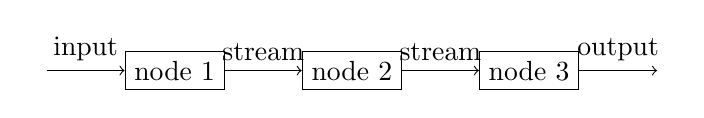
\begin{tikzpicture}[node distance=2.25cm, ->]
\node (S) {};
\node (A) [draw, right of=S, node distance=1.75cm] {node 1};
\node (B) [draw, right of=A] {node 2};
\node (C) [draw, right of=B] {node 3};
\node (E) [right of=C, node distance=1.75cm] {};
\path (S) edge node[above] {input} (A);
\path (A) edge node[above] {stream} (B);
\path (B) edge node[above] {stream} (C);
\path (C) edge node[above] {output} (E);
\end{tikzpicture}
\end{center}


In order to expose data parallelism from the output of a command,
files that don't point to a resource can have an upper bound on the
lines that they can tranfer. The following example illustrates why
this is essential.

\TODO{Add an example of a command that has two outputs, one of which
  goes to one command, while another goes to a different
  command. Maybe only show the graph here and not the command itself.}


\tr{On the other hand, some forms of data parallelism can be exposed
  when knowing the size of the input files. As mentioned in \ref{}
  some pure commands (such as cat -n) only need line information to
  become stateless, and knowing the size of a file could allow the
  system to split it in different chunks that can be processed
  independently. To account for that, edges that refer to an input
  resource contain the number of lines of the file that they refer
  to.}

Finally, the edges that don't refer to a resource and do not start
from a node in the graph represent the graph input, while the edges
that don't refer to a resource and do not point to a node in the graph
are its outputs.

\kk{(Maybe) It might be beneficial to mention that many inputs do not
  represent the same thing as many outputs. These two notions are not
  symmetric.}
  
\begin{figure*}
\centering
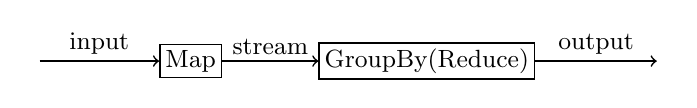
\begin{tikzpicture}[->, >=to, auto, node distance=1cm, semithick, transform shape, inner sep=2pt]
%
\small
%
\node (M1) {};
\node (M2) [draw, right of=M1, node distance=2cm] {Map};
\node (M3) [draw, right of=M2, node distance=3cm] {GroupBy(Reduce)};
\node (M4) [right of=M3, node distance=3cm] {};
%
\path (M1) edge node {input} (M2);
\path (M2) edge node {stream} (M3);
\path (M3) edge node {output} (M4);
\end{tikzpicture}
\end{figure*}

\begin{figure*}
\newcommand{\Split}{\text{Split}}
\newcommand{\Merge}{\text{Merge}}
\newcommand{\Map}{\text{Map}}
\newcommand{\GroupBy}{\text{GroupBy}}
\newcommand{\Reduce}{\text{Reduce}}
\centering
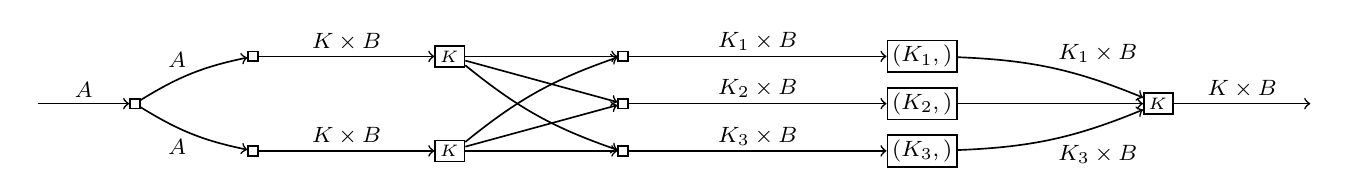
\begin{tikzpicture}[->, >=to, auto, node distance=0.6cm, semithick, transform shape, inner sep=1.75pt]
%
\footnotesize
%
\node (M1) {};
\node (M2) [draw, right of=M1, node distance=1.3cm] {$\Split$};
\node (M3) [right of=M2, node distance=1.5cm] {};
\node (M4) [right of=M3, node distance=2.5cm] {};
\node (M5) [draw, right of=M4, node distance=2.2cm] {$\Merge$};
\node (M6) [draw, right of=M5, node distance=3.8cm] {$\GroupBy(K_2,\Reduce)$};
\node (M7) [draw, right of=M6, node distance=3cm] {$\Merge_K$};
\node (M8) [right of=M7, node distance=2cm] {};
%
\node (T3) [draw, above of=M3] {$\Map$};
\node (T4) [draw, above of=M4] {$\Split_K$};
\node (T5) [draw, above of=M5] {$\Merge$};
\node (T6) [draw, above of=M6] {$\GroupBy(K_1,\Reduce)$};
%
\node (B3) [draw, below of=M3] {$\Map$};
\node (B4) [draw, below of=M4] {$\Split_K$};
\node (B5) [draw, below of=M5] {$\Merge$};
\node (B6) [draw, below of=M6] {$\GroupBy(K_3,\Reduce)$};
%
\path (M1) edge node {$A$} (M2);
\path (M2) edge[bend left=10] node {$A$} (T3);
\path (M2) edge[bend right=10] node[swap] {$A$} (B3);
\path (M5) edge node {$K_2 \times B$} (M6);
\path (M6) edge (M7);
\path (M7) edge node {$K \times B$} (M8);
%
\path (T3) edge node {$K \times B$} (T4);
\path (T4) edge (T5);
\path (T4) edge (M5);
\path (T4.330) edge[bend right=10] (B5.170);
\path (T5) edge node {$K_1 \times B$} (T6);
\path (T6) edge[bend left=10] node {$K_1 \times B$} (M7);
%
\path (B3) edge node {$K \times B$} (B4);
\path (B4) edge (B5);
\path (B4) edge (M5);
\path (B4.30) edge[bend left=10] (T5.190);
\path (B5) edge node {$K_3 \times B$} (B6);
\path (B6) edge[bend right=10] node[swap] {$K_3 \times B$} (M7);
%
\end{tikzpicture}
\caption{Distributed implementation of the map-reduce pipeline $\Map \gg \GroupBy(K,\Reduce)$.}
\label{fig:mapReduce}
\end{figure*}



\subsection{Graph transformations}
\label{ir:transformations}

As mentioned above, the dataflow graph exposes task
parallelism. Different nodes in the graph can be executed
concurrently, communicating through the edges. Task level parallelism
is already exposed by the shell, by using pipes \ttt{|} and the
background operator \ttt{\&}. Unfortunately, simple task
parallelism leaves a lot to be desired, since scaling a computation
requires manually introducing more operators.

In order to adequately utilize the available computational resources,
a distributed implementation should exploit data parallelism. Data
parallelism is based on the observation that some operations produce
the same result when performed independently on subsets of the input
data, merging the results afterwards. This is the basic optimization
that is used by popular distributed processing systems such as
MapReduce \cite{DG2004MR} and Apache Spark \cite{spark:12}. Unfortunately, the
dataflow graph model of most of these systems is not expressive enough
to represent data parallelism \km{not sure this is true}, so the distributed implementations that
they perform do not preserve the semantics of their dataflow model.

In contrast, our dataflow model inherently supports the data
parallelism that is found in shell programs. More precisely, data
parallelism can be easily exposed as task parallelism in our model. A
very important consequence of this is that we can iteratively apply
optimizations that expose data parallelism, or even revert them when
the resulting dataflow graph is too wide. This flexibility enables
unified reasoning and implementation of the unoptimized and optimized
version of the dataflow graph. \kk{This is interesting, and should be
  moved up (or rephrased in the introduction)}

Before describing the different types of parallelization
optimizations, we formalize the intuition about stateless and pure
commands that was described in \Cref{cmd}.
\nv{TODOs
  (i) highlight earlier the antithesis between the formalisms in this section and the informalities of the previous (me);
  (ii) try to add a proof \emph{sketch} pointing to these formalisms (to show their value), and we can point to the TR for the longer proof.
}
%
As mentioned there, stateless commands operate independently on
individual elements of the stream (characters, lines, or files)
without maintaining any state. Some examples include \ttt{grep},
\ttt{basename}, and \ttt{tr}. Formally, a commmand $f$ is stateless if
it is ``linear'' with respect to concatenation, i.e. the following
equation holds:

\[
\forall x, x', f(x.x') = f(x).f(x')
\]

\km{This is a nice characterization, which I think is true in most settings. There is a caveat though: You can have stateless programs that emit output when they start (before they consume the stream) and/or when they consume the EOF symbol. In this case I am not sure the equation above holds.}

Similarly, it was mentioned that some pure commands (such as
\ttt{sort} and \ttt{wc}) can be parallelized using divide-and-conquer
techniques. More formally, there pure commands $f$ can be implemented
as a map $m$ and a reduce $r$ function, satisfying the following:

\[
\forall x, x', f(x.x') = r(m(x).m(x'))
\]

\heading{Parallelization Transformations}
%
Based on these equations, we can define a maximal \emph{node split
  operation} on a stateless node $v$ with $n$ input ordered edges and
an output edge to node $v'$, to replace $v$ with $n$ new nodes, giving
each one of them one of the incoming edges of $v$, and routing them in
order to point to $v'$. Since each incoming edge represents a stream
of data $x_i : D^*$, and the only behaviour of a dataflow graph is its
output, this optimization $ v(x_1.x_2...x_n) \Rightarrow
v(x_1).v(x_2)...v(x_n)$ can be shown to preserve the behaviour of the
graph. Furthermore, it can be straightforwardly extended to pure
commands that can be implemented by a map-reduce pair $(m, r)$ as $
v(x_1.x_2...x_n) \Rightarrow r(m(x_1).m(x_2)...m(x_n))$.

\tr{Remember to mention the assumptions that need to hold for the
  graph transformations to be valid in the Command categories
  section. Commands must be deterministic, they must not do any other
  side effect (such as writing to other files, sending signals,
  etc). However, these assumptions must already be checked when the
  developer designates the categories.}

\tr{If there is time I can work out a formal definition and a proof
  sketch why this transformation preserves the output of the dataflow
  graph.}

%% \begin{definition}
%% Given a dataflow graph $G = (V, E, O)$, where $V$ is a set of nodes
%% representing commands, $E$ is a set of edges representing files, and
%% $O$ is a function from $V \cup v_{out}$ to a total order of incoming
%% edges. $v_{out}$ represents a concatenation of all the outputs of the
%% dataflow graph. We represent the total order for a node $v$ as
%% $<_v$. Given a node a node $v$
%% with input edges $ie = \{ i_1 = (v_{i_1}, v, 1), i_2, ..., i_n =
%% (v_{i_n}, v, n) \}$ and output edge $o = (v, v_o, a)$, we define a
%% complete node split $s(v, G) = (V', E')$ where $V' = V - v \cup \{
%% v_1, ..., v_n \}$ and $E' = E - ie \cup \{(v_{i_1}, v_1, 1), ...,
%% (v_{i_n}, v_n, 1) \} - o \cup \{ (v_1, v_o\}$
%% \end{definition}

%% \begin{lemma}
%% tofill
%% \end{lemma}

In addition to node splits, we can also perform edge splits in order
to increase the number of incoming edges for some nodes to expose
possible data parallelism. If the edge refers to a real file, then the
edge split represents splitting the real file in chunks, while in
cases where the edge connects two nodes, it is split to several edges
with a bounded number of lines. Note that the final output edge of a
valid node in the graph must always be unbounded if it does not refer
to a file.





\section{Implementation}
\label{impl}

As mentioned in \Cref{ir}, in order to generate the distributed
implementation of a shell script, \ttt{Dish} first translates it to
a dataflow graph. However, there are several components in shell
programs that cannot be arbitrarily parallelized without affecting the
program behaviour, e.g. commands producing an irreversible effect, or
commands connected with a \ttt{\&\&} operator. In addition, the
fact that the shell is \todo{extremely dynamic}, further increases the
challenge of correctly identifying what parts can be distributed.

%% \kk{Give examples of writing to environment variables, producing
%%   irreversible side effects, the ; and \&\& operators.}

In order to address this issue, we \todo{introduce} the notion of
distributable program regions, and we design a translation pass that
given the abstract syntax tree of a shell script identifies
distributable regions and translates each of them to a dataflow
graph. The AST of the shell script is produced using a POSIX compliant
parser~\cite{libdash}.

\subsection{Distributable Regions}

%% \kk{The goal of this subsection is to explain that Dish does a safe
%%   but effective analysis to identify which parts of the scripts to
%%   parallelize.}

Consider the following example:

\begin{lstlisting}[language=sh, float=h, numbers=none, escapeinside={($}{$)}]
  cat f1 f2 | grep ``foo'' > f3 &&
  sort f3 # Replace with sth better
\end{lstlisting}

\noindent
Notice that the structure of a shell program can be used to identify
components that can be executed concurrently, and barriers that
enforce synchronization. More precisely, \ttt{cat f1 f2} and \ttt{grep
  ``foo''} would already execute concurrently in the standard shell,
while \ttt{sort f3} would wait for their completion before being
executed. Both \ttt{cat f1 f2 | grep ``foo'' > f3} and \ttt{sort f3}
are maximal distributable regions, in the sense that they cannot be
extended beyond \ttt{\&\&}.

Concretely, a distributable region cannot permeate through barrier
constructs (e.g. \ttt{;}, \ttt{\&\&}, and function definitions). On
the other hand, the pipe operator \ttt{|} and the parallel composition
operator \ttt{\&} enable parallelization, and extend distributable
regions. Intuitively, distributed regions correspond to subsections of
the program that would be allowed to execute concurrently by different
processes in the POSIX standard~\cite{posix}.

\tr{I don't know whether I should mention the following: While these
  control flow constructs can be parallelized and there has been
  research on it, it is orthogonal to our work, and can be
  incorporated as future work.}

\subsection{Translation Pass}

Dish performs a depth first search pass on the AST of the given shell
program, extending the distributable regions from the bottom up,
translating their independent components to dataflow graph
nodes, until a barrier construct is reached. Note that barrier
constructs can exist in a dataflow graph, as long as they don't
extend beyong a single node. An illustrative example follows:

\begin{lstlisting}[language=sh, float=h, numbers=none, escapeinside={($}{$)}]
  (sort f1 > g1 && sort f2 > g2) &
  sort -m g1 g2
\end{lstlisting}

In the above example, while \ttt{sort f1 > g1}, \ttt{sort f2 > g2},
and \ttt{sort -m g1 g2} are all in different dataflow graphs, the
dataflow graph that corresponds to the whole program, has two nodes,
\ttt{sort f1 > g1 \&\& sort f2 > g2} and \ttt{sort -m g1 g2}.

In order to identify possible opportunities for parallelism, the
translation pass also identifies the category of each node, together
with its input and output, using records written by developers using
the language that was described in \Cref{ext}. Some interesting cases
of the analysis algorithm are shown in pseudocode below:

\begin{lstlisting}[language=python, float=h]
  def translate(node):
    ...
    elif(node.name == 'Pipe'):
      return pipe_graphs([translate(child)
        for child in node.children])
    elif(node.name == 'And'):
      node.children = [translate(child)
        for child in node.children]
      return node
    elif(node.name == 'Command'):
      if(not safe(node)):
        return make_ir_node(node, 'unsafe')
      else:
        return make_ir_node(node,
          find_category(node))
    ...
\end{lstlisting}

Whenever the algorithm encounters a pipe node, it recursively
translates its subcomponents, and then merges them in a dataflow graph
by connecting the output of the first with the input of the second,
\etc. Before the different dataflow graphs are connected, the
algorithm checks that at most one node in the graph writes at every
file, and at most one node reads from a file that another node writes
to. This is important, in order to avoid inconsistent behaviour after
distributing nodes in the dataflow graph (i.e. by introducing to
concurrent reads and writes to the same file when
parallelizing). Whenever the algorithm encounter an \ttt{\&\&} node,
it recursively translates its subcomponents (similarly to the pipe
node), but then does not merge them in a large dataflow
graph. Finally, whenever the algorithm encounters a command, it first
checks whether it is safe to parallelize it. A command is considered
to be safe, if it does not make any modification to the shell state
(e.g. changing the current directory, modifying environment
variables), and if it does not read from any \todo{read-once} file,
like a fifo pipe. If the command is considered safe, its category is
identified and a node containing that command is created and added to
a singleton dataflow graph. If the command is considered unsafe, it is
still added to the dataflow graph, but cannot be further parallelized
by the optimizer.

An important consideration is that due to the highly dynamic nature of
the shell, the safety properties that are mentioned above cannot be
soundly checked statically. For example in the first case, two
unexpaned strings could refer to the same file, but the translation
pass cannot infer that.

\subsection{Dish Optimizer}

The \ttt{Dish} optimizer is given a dataflow graph representing a
shell program and outputs an optimized dataflow graph, where data
parallelism opportunities have been exploited. More concretely, the
optimizer starts by splitting input files in several chunks, given the
desirable output dataflow graph width. It then starts from the source
nodes of the graph, iteratively performing the graph transformations
that were described in \Cref{ir:transformations}. If the incoming
edges of the node are less than the desirable graph width, it performs
edge splits, and then it performs maximal node splits. The final graph
can then be implemented by spawning a process for each node, and
redirecting the outputs according to the graph edges.

\nv{Give example, extend}


%% \subsection{Mapping operators to nodes}

%% \kk{I don't think we should mention this.}

%% Explain the simple algorithm that we used to minimize intra node
%% communication, that tries to map contiguous parts of the graph to the
%% same node. We could do this by having an algorithm that minimizes the
%% number of cuts or something.

%% We don't try to make a proper planner, as there is a lot of work on
%% operator placement etc. that we can borrow from.

\subsection{Planning Activators and Just-in-Time Planning}

\nv{Nikos working on this and next}

% \kk{This whole section for just in itme planning, is also relevant for
%   the front end. If the front end is executed just in time, it would
%   have more information, and maybe it could make a sound analysis.}

Important point: Shell is extremely dynamic. Because of this, a
distributor cannot decide how to distribute a subexpression
statically, by just reading the script, (as in many other systems like
MapReduce, Spark, etc), since most of the information is not there
before the script starts executing. Environment variables,
unexpanded(unevaluated) strings \kk{Make sure that terminology is
  consistent with Greenberg}, could all contain information that is
valuable to make the distribution plan \kk{give an example}.


Future work on this: calling the shell shtepper to only partially
evaluate strings, just expand arguments, and not do any significant
computation. Even better, we could be calling the shtepper just after
having parsed the ast, and decide on maximal distributable subtrees as
late as possible in the process. This would be awesome.

\subsection{Merge and Split Implementation}

It is common in the dataflow graph for a node to have many incoming
edges, or many outgoing edges (when all but the last outgoing edges
are bounded). However some nodes, might only read their input from one
source (e.g. stdin). In this case, the distributed implementation
needs to concatenate input files (or conversely split output
files). Here is an example:

\kk{Show an example graph! of cat | tr | sort. The command in the
  middle must only take input from one file (maybe just stdin).}

We address this issue using primitive shell constructs for file
manipulation. More concretely a merger can be implemented by a simple
\verb|cat|. Given a set of input files \verb|in1, in2, ...| and an
output file \verb|out|, a merger can be implemented as:

\begin{lstlisting}[language=sh, float=h, numbers=none]
 cat $in1 $in2 ... > $out
\end{lstlisting}

\noindent
\TODO{Change that with the new splitter}
On the other hand, given an input file \verb|in| that is a FIFO pipe,
and two output files \verb|out1, out2| the first of which is bounded
to \verb|N| lines, a 2-splitter can be implemented as:

\begin{lstlisting}[language=sh, float=h, numbers=none]
 head -n $N $in > $out1 ; cat $in > $out2
\end{lstlisting}

\noindent
Using the 2-splitter as a building block, a pipe can be split to
arbitrarily many different pipes.


\section{Evaluation}
\label{eval}

% FIXME
% \kk{We should make sure to measure the time that it takes for the
%   whole process to run (parsing, translating, optimizing, planning)
%   together with the scripts. This will probably be negligible, but we
%   still have to mention it. }
% 
% \kk{Also, we have to have one-two handcrafted examples that have more
%   than one pipeline, to show the execution time end to end, as this
%   cannot be shown with the one-pipeline examples since they only have
%   one graph, so no back and forth between shell and dish.}
% 
% \kk{Furthermore it would be great to have one distributed example that
%   runs in more than one node (if we have time)}
% 
% \kk{Also we have to make sure to measure with and without the final
%   cat of output file, so that we show that this is also negligible.}
% 
% \kk{We have to make sure that we repeat that the results are the same
%   in all tests that we run. Corectness, blah blah ...}
% 
% \kk{We should have at least some pipelines that have a bad pure
%   command in them.}

\begin{table*}[t]
\center
\footnotesize
% \setlength\tabcolsep{3pt}
\caption{
  \footnotesize{
    \textbf{Summary of Micro-benchmarks}.
    The micro-benchmarks are small pipelines (\ie ones developed on-the-fly) drawn from various sources and applied to large datasets.
  }
}
\begin{tabular*}{\textwidth}{l @{\extracolsep{\fill}} llllll}
\toprule
  Script                 ~&~ Structure                    & Input (MB)& Time (Seq)    & Script Size (LoC)             & Highlights                                        \\
\midrule
% https://github.com/andromeda/sdsh/blob/master/scripts/grep.sh
  \tti{min-grep}         ~&~$3\times$\tsta                &           &               &   17\qquad 134\qquad  1304    & complex NFA regex                                 \\
% https://github.com/andromeda/sdsh/blob/master/scripts/minimal5.sh
  \tti{min-sort}         ~&~~$\tsta, \tpur$               &           &               &   X \qquad 129\qquad  1209    & \tti{sort}ing                                     \\
% https://github.com/andromeda/sdsh/blob/master/scripts/topn.sh
  \tti{wf}               ~&~~$3\times\tsta, 3\times\tpur$ &           &               &   X \qquad 181\qquad  1621    & double \tti{sort}, \tti{uniq} reduction           \\
% https://github.com/andromeda/sdsh/blob/master/scripts/topn.sh
  \tti{top-n}            ~&~~$2\times\tsta, 4\times\tpur$ &           &               &   X \qquad 181\qquad  1621    & double \tti{sort}, \tti{uniq} reduction           \\
% https://github.com/andromeda/sdsh/blob/master/scripts/ngrams.sh
  \tti{bi-gram}          ~&~~$2\times\tsta, 4\times\tpur$ &           &               &   X \qquad  X \qquad          & stream shifting and merging                       \\
% https://github.com/andromeda/sdsh/blob/master/scripts/spell.sh
  \tti{spell}            ~&~~$4\times\tsta, 3\times\tpur$ &           &               &  37 \qquad 257\qquad  2417    & comparisons (\tti{comm})                          \\
% https://github.com/andromeda/sdsh/blob/master/scripts/diff.sh
  \tti{diff}             ~&~~$4\times\tsta, 3\times\tpur$ &           &               &   X \qquad  X \qquad          & shuffling and non-distributable \tti{diff}ing     \\
\bottomrule
\end{tabular*}
\label{tab:eval}
\end{table*}


At a high level, we are interested in understanding whether \sys can indeed scale pipelines out automatically and correctly.
To achieve this, we use a combination of micro- and macro-benchmarks, most of which were collected from prior literature and online repositories.
Micro-benchmarks~\sx{micro} are one-off, simple one-line pipelines that take a few seconds to write (usually interactively);
  such pipelines are usually composed interactively to solve a task at hand, test a hypothesis, or ``smoke out bugs''~\cite{bentley1986literate}---but, with \sys, applied to very large data sets.
These pipelines are taken from real use cases (often from the literature~\cite{bentley1985spelling, bentley1985spelling}), and, precisely due to their small size, have the benefit of highlighting stress on a handful of stages.

Three complex macro-benchmarks (\S\ref{macro1}--\ref{macro3}) involve third-party commands and handle realistic workloads by today's standards.
These scripts are about an order of magnitude larger than the micro-benchmarks, but this perceived lack of complexity is deceiving:
  as shown below, if written in conventional languages, these pipelines would correspond to programs on the order of hundreds of lines of code.

Several results are worth highlighting.
First and foremost, programs see a significant speedup, often more $10\times$ over sequential execution  while returning identical results (on very large datasets).
\sys's transformation and planning phase take around XX--XXms, negligible (XX\%) for short-running pipelines and virtually non-existent for long-running ones.
As \sys rewrites to highly-optimized shell primitives rather than using a managed language runtime, it always has a COST~\cite{mcsherryscalability} of 2.
Finally, \sys preserves the productivity of the shell:
  in one case, the equivalent program for a small part of the pipeline requires over a 150 lines of code in combined Java and Bash to run distributed on top of Hadoop;
  in another, the program expressed by the pipeline was the subject of a semester project in a graduate course on distributed systems~\cite{blinded} where student implementations ranged between 1--3\textbf{K} lines of code.

Experiments were run on a %\todo{network of five workstations} connected by 1Gbps links: 
 machine with 512GB of memory and 128 2.1GHz Intel Xeon E5-2683 cores.
%\todo{four smaller machines (\wkq), each with 4GB of memory and two 3.33GHz Intel Core Duo E8600 processors}.
For our software setup, we use SMP Debian 4.9.144-3.1 (2019-02-19), GNU Core-utils 8.30-3, GNU Bash 5.0.3(1)-release (x86\_64-pc-linux-gnu), Python 3.7.3, and OCaml 4.05.0.
Generally, no special configuration was made in hardware or software beyond disabling hyper-threading. % ---specifically, the network protocol stack was left unoptimized.
All pipelines are set to (initially) read from and (finally) write to the file-system (except as otherwise stated).
Whenever \ttt{curl} is part of a pipeline, it fetches data from a different physical host on the same network connected by 1Gbps links.
More detailed setup and experiments, including the scripts, is included in the accompanying (anonymized) online repository.

\subsection{Microbenchmarks: Shell One-liners}

\begin{figure*}[t]
    \centering
    %% \subcaptionbox{\label{eval:minimal_grep}}{
    %%     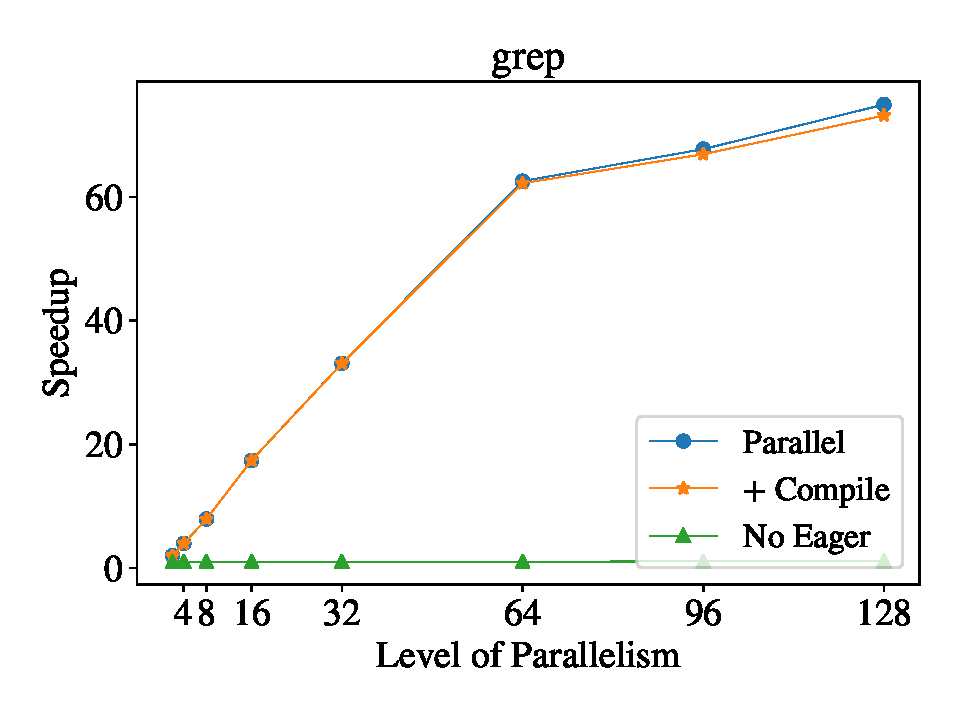
\includegraphics[width=0.32\textwidth]{\detokenize{./figs/minimal_grep_throughput_scaleup.pdf}}
    %% }
    %% \subcaptionbox{\label{eval:grep}}{
    %%     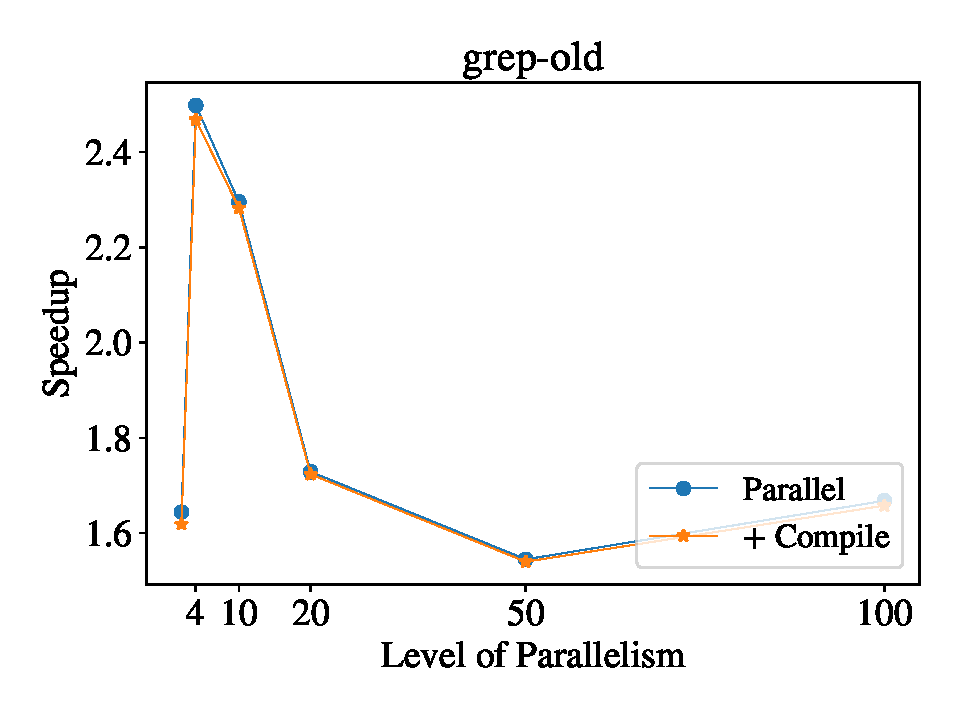
\includegraphics[width=0.32\textwidth]{\detokenize{./figs/grep_throughput_scaleup.pdf}}
    %% }
    %% \subcaptionbox{\label{eval:minimal_sort}}{
    %%     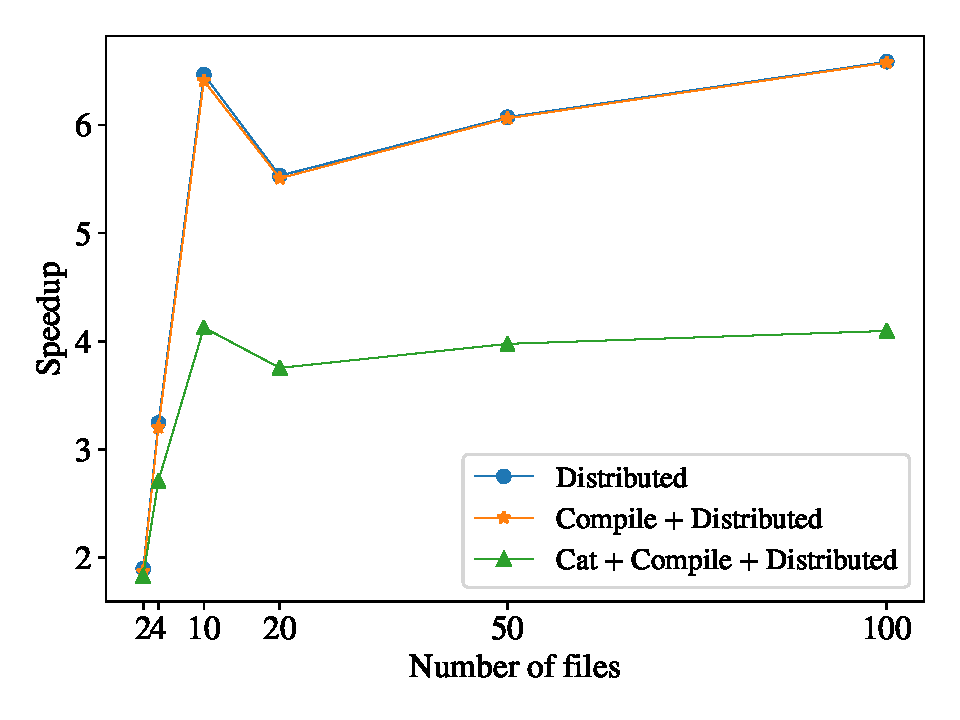
\includegraphics[width=0.32\textwidth]{\detokenize{./figs/minimal_sort_throughput_scaleup.pdf}}
    %% }
    %% \subcaptionbox{\label{eval:topn}}{
    %%     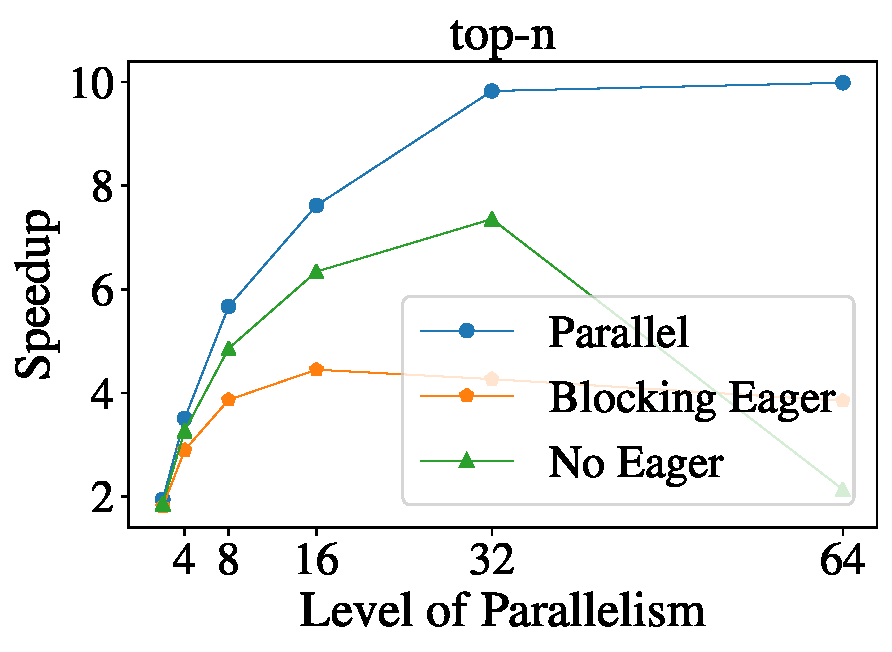
\includegraphics[width=0.32\textwidth]{\detokenize{./figs/topn_throughput_scaleup.pdf}}
    %% }
    %% \subcaptionbox{\label{eval:wf}}{
    %%     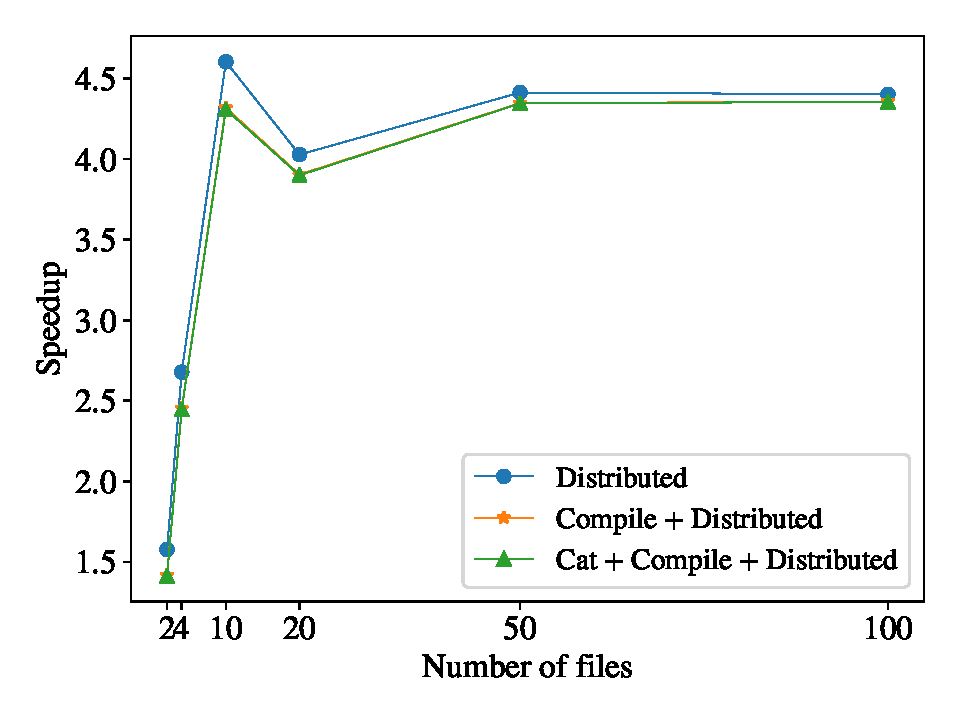
\includegraphics[width=0.32\textwidth]{\detokenize{./figs/wf_throughput_scaleup.pdf}}
    %% }
    %% \subcaptionbox{\label{eval:spell}}{
    %%     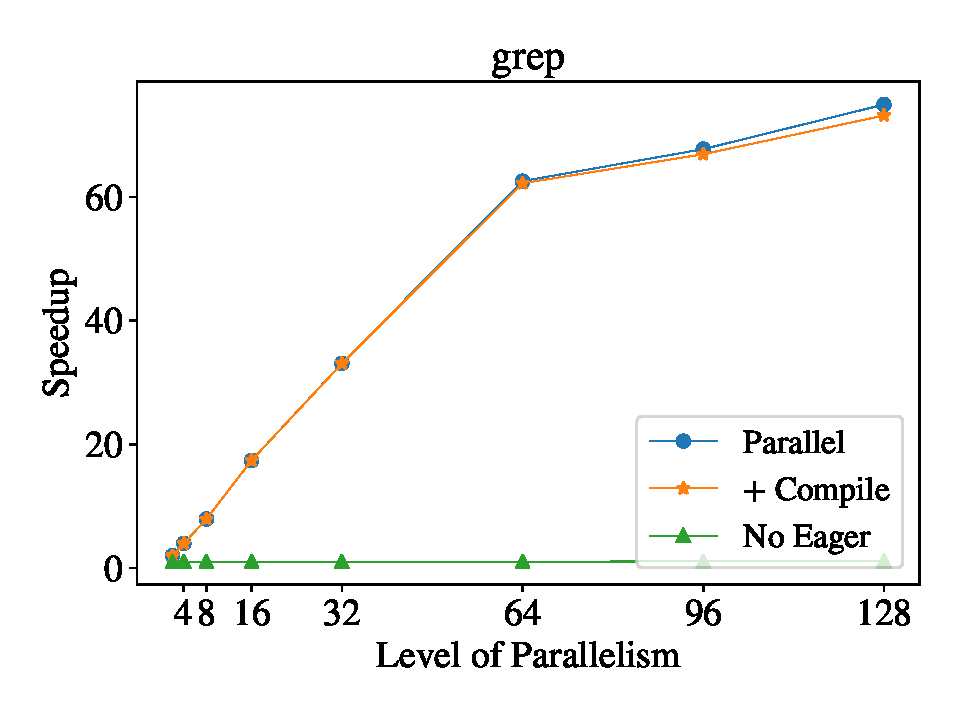
\includegraphics[width=0.32\textwidth]{\detokenize{./figs/minimal_grep_throughput_scaleup.pdf}}
    %% }
    %% \caption{a}
    \begin{subfigure}[b]{0.32\textwidth}
        \centering
        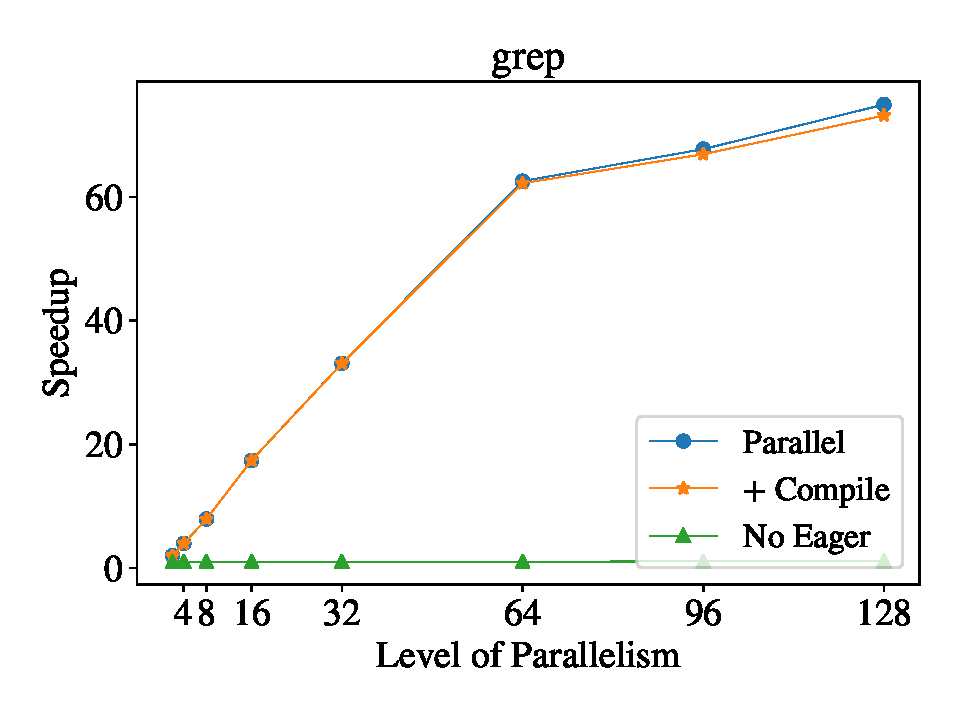
\includegraphics[width=\textwidth]{\detokenize{./figs/minimal_grep_throughput_scaleup.pdf}}
        %% \caption{TODO}
        %% \label{eval:minimal_grep}
    \end{subfigure}%
    ~
    \begin{subfigure}[b]{0.32\textwidth}
        \centering
        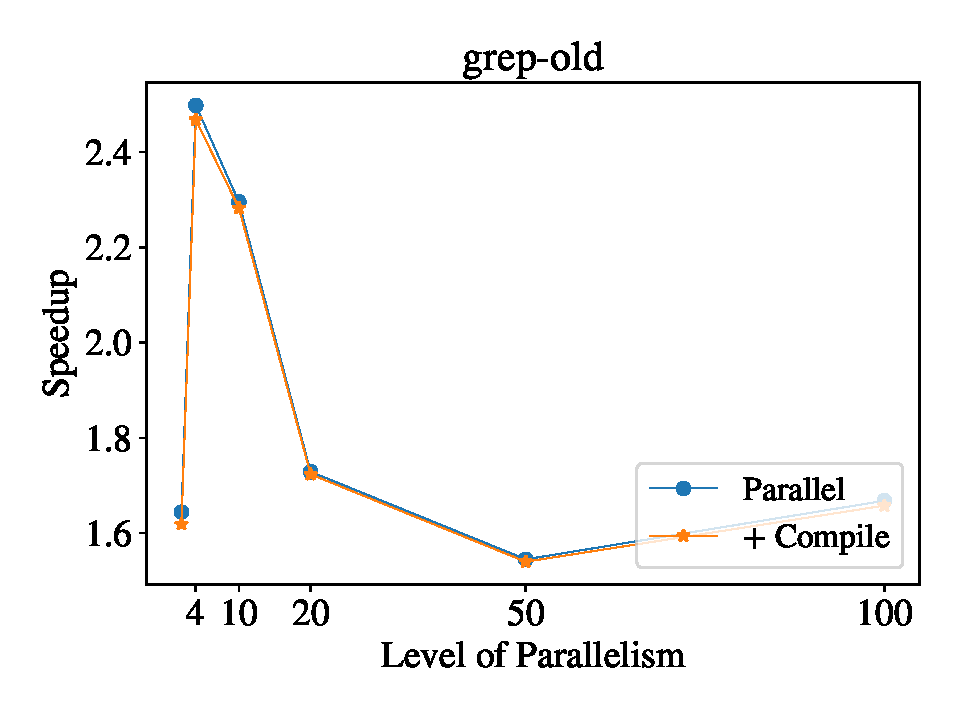
\includegraphics[width=\textwidth]{\detokenize{./figs/grep_throughput_scaleup.pdf}}
        %% \caption{TODO}
        %% \label{eval:grep}
    \end{subfigure}%
    ~
    \begin{subfigure}[b]{0.32\textwidth}
        \centering
        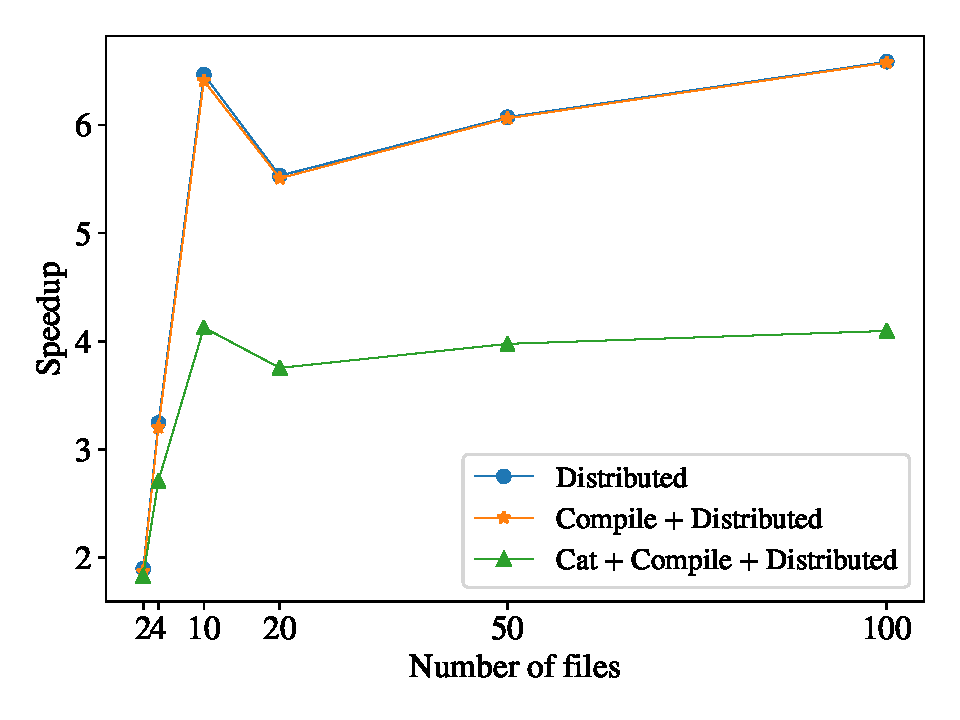
\includegraphics[width=\textwidth]{\detokenize{./figs/minimal_sort_throughput_scaleup.pdf}}
        %% \caption{TODO}
        %% \label{eval:minimal_sort}
    \end{subfigure}%

    \begin{subfigure}[b]{0.32\textwidth}
        \centering
        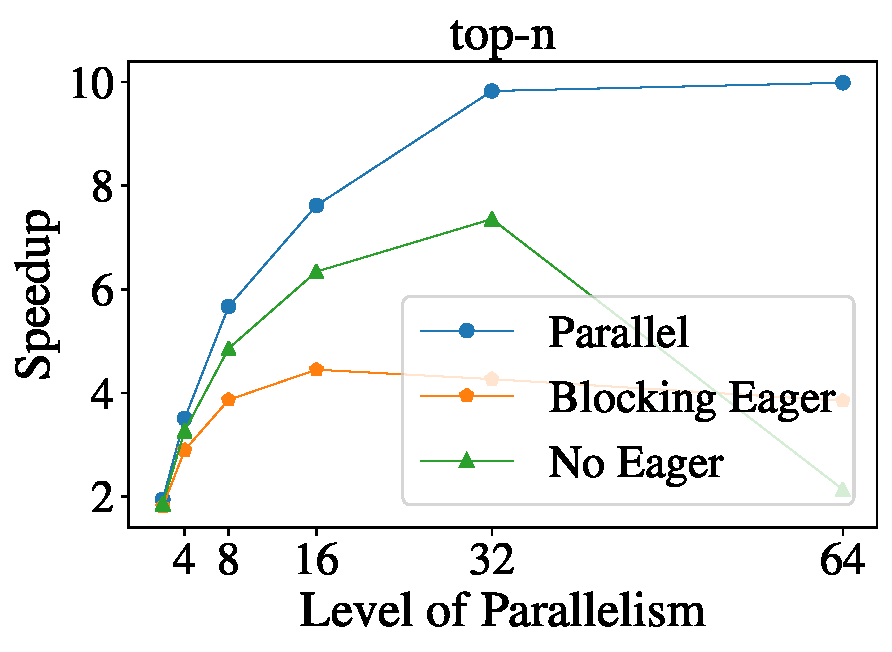
\includegraphics[width=\textwidth]{\detokenize{./figs/topn_throughput_scaleup.pdf}}
        %% \caption{TODO}
        %% \label{eval:topn}
    \end{subfigure}%
    ~
    \begin{subfigure}[b]{0.32\textwidth}
        \centering
        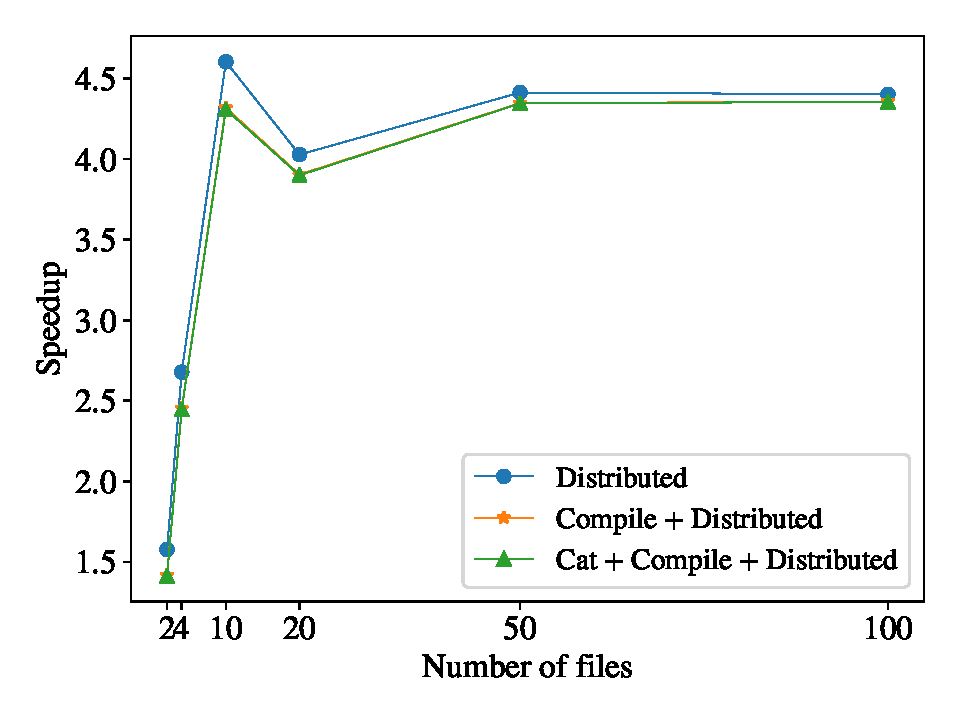
\includegraphics[width=\textwidth]{\detokenize{./figs/wf_throughput_scaleup.pdf}}
        %% \caption{TODO}
        %% \label{eval:wf}
    \end{subfigure}%
    ~
    \begin{subfigure}[b]{0.32\textwidth}
        \centering
        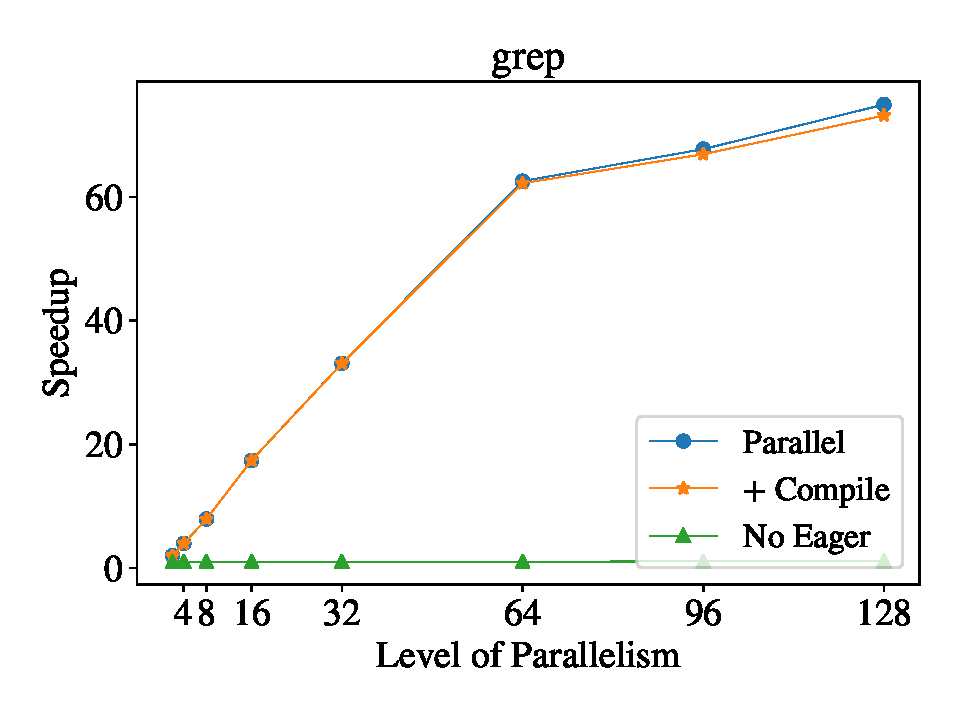
\includegraphics[width=\textwidth]{\detokenize{./figs/minimal_grep_throughput_scaleup.pdf}}
        %% \caption{TODO}
        %% \label{eval:spell}
    \end{subfigure}%
    \caption{
      \textbf{Speedup achieved by \sys as a function of the level of parallelism (1--200).} 
Three different configurations per benchmark:
  (i) distributed, focusing only on the distributed execution,
  (ii) +compile, adding \sys' pre-processing overheads, and
  (iii) +cat, adding a final merger step.
    }
    \vspace{-15pt}
    \label{fig:microbenchmarks}
\end{figure*}


Tab.~\ref{tab:eval} summarizes the collection of micro-benchmarks used to evaluate \sys.
Benchmark names (col. 1) correspond to the names on the plots (Fig.~\ref{fig:microbenchmarks}).
% The centralized pipelines read files of various sizes from disk and write to disk.

Input sizes and times (col. 2, 3) summarize the longest sequential execution (200 files in Fig.~\ref{fig:microbenchmarks}).
Script sizes report on the \sys's rewritten output for three different distribution sizes---$1\times$, 10$\times$, and $100\times$.

The size of a script (col. 5) grows due to the resulting complexity of coordinating among parallel executions---multiple FIFOs per pipeline stage, merging and splitting, encoding of divide-and-conquer synchronization \etc
The first number alone is interesting, as it captures \sys's output for the sequential script.
As there is no parallelism, it can be viewed as the initial cost corresponding to using \sys.
% this is the size of 
This change in size does not necessarily translate to observed runtime, as most of this size gain comes from the setup and teardown of FIFOs responsible for interprocess (IPC) communication.
FIFOs are simply pipes made, the in-kernel buffering and synchronization mechanisms are the same, leading to non-observable changes in runtime performance.

In terms of benchmarks, \ttt{grep} is a short script centered around an expensive \sta command.
% a DFA-based regular expression matching phase;
  while \ttt{grep} defaults to a Thompson NFA, this particular expression makes use of DFA-based backtracking patterns resulting in high runtime overhead.
The \ttt{sort} pipeline is equally short, but its central operation is a command in \pur.
The next two benchmarks, \ttt{wf} and \ttt{top-n}, are based on McIlroy's now classic word-counting program~\cite{bentley1986literate};
  they use sorting, rather than tabulation, to identify high-frequency terms in a corpus.
The \ttt{bi-gram} pipeline calculates n-grams of base two;
  it makes clever use of \ttt{tail} to shift a stream by one word and \ttt{paste} to fuse (zip) two streams together.
The next pipeline is based on the original \ttt{spell} program developed by Johnson~\cite{bentley1985spelling}---another \unix classic:
  after some preprocessing, it makes clever use of \ttt{comm} to report words not in the dictionary.

% TODO \nv{Need to change terminology in plots---files should be (attempted) parallelism, name benchmark, cat should be merge.}
Fig.~\ref{fig:microbenchmarks} presents the speedup gained by \sys as a function of the level of parallelism (1--200).
% we experiment with a $200\times$ level of parallelism to see potential overheads
Each one of these plots reports on three different configurations:
  (i) distributed, which captures only the runtime of the distributed computation,
  (ii) compile + distributed, which adds the \sys' analysis and generation overhead, and
  (iii) cat + compile + distributed, which adds a final merger  gathering the results at the end of the pipeline.
The results show significant speedups, ranging between \todo{7--70$\times$}, depending on the distributability characteristics of individual pipelines.

Interestingly, the overhead from \sys's analysis and generation phases remains collectively below 1s even for the high-scalability cases.
We decided to push \sys's limits of these phases by synthesizing an artificial 1000-stage pipeline---a carefully-constructed, worst-case workload that is nowhere near the ones observed in practice (\S\ref{macro1}--\ref{macro3}).
We find the resulting times quite acceptable:
  \todo{8.23s} for parsing the script, 
  \todo{3.22s} for analysis, and 
  \todo{X.XXs} for rewriting the results of the analysis.

\subsection{Macro-benchmark: Weather Analysis}
\label{macro1}

For \sys's first macro-benchmark, we use we
from introductory chapter of Hadoop Definitive Guide~\cite[Chapter 2]{hadoop:15}
This example is used as a data analysis Hadoop is well suited for, and combines the 
There are several interesting aspects about this case.
First, Hadoop is used 
McIlroy would have probably expressed---our pipeline 
14 stages long;

The effort required to write this pipeline is astonishingly low:
  it amounts to 240 characters 
(Some effort is required to understand NCDC's weather format, but this is true for any program processing this dataset.)

The pipeline starts with a few stages in \sta  that generate URLs;
  these URLs point to index files, each one of which contains pointers 
The stream of index files is analyzed (4 stages) to extract the URLs of the compressed data files.
It is then passed again through a download command
After downloading and uncompressing these files, the stream is analyzed to extract the maximum temperature.

A less obvious lesson from this case was that  
First, large, complex pipelines enable significant freedom in how to express some stages.
Several stages in the original program are compressed into a single \ttt{awk} script;
  unfortunately, \ttt{awk} is too general to have a helpful distributability signature.
For example, the \ttt{sort} command at the end is an expensive version of extracting the maximum element;
  this could have been expressed with a simple \ttt{awk} script that only keeps track of the max.

The Hadoop program 
Hadoop 3.2.1
openjdk 11.0.5
ruby 2.5.5p157

few different ways to write some phases, 
  for example, 
A large pipeline resulted in a couple of 
An interesting lesson here was that there are multiple
First, longer pipelines can be written in multiple ways
It is worth noting
These are 

% /home/nikos/hadoop-3.2.1/bin/hdfs dfs -put /home/nikos/dish/scripts/max-temp 77.24s user 50.79s system 185% cpu 1:09.14 total
% hadoop jar $HADOOP_HOME/share/hadoop/tools/lib/hadoop-streaming-*.jar -input 719.26s user 63.88s system 155% cpu 8:22.47 total

\subsection{Macro-benchmark: Bioinformatics Transform}
\label{macro3}

\subsection{Macro-benchmark: Web Crawling}
\label{macro2}

\section{Related Work}
\label{related}

At a high-level, techniques for automatically distributing fall under a spectrum that ranges from fully automated (but potentially sub-optimal) distribution to fully manual (but, ideally, optimal) distribution (Fig.~\ref{fig:spectrum}).

% Nice intro: http://homepages.inf.ed.ac.uk/bfranke/Publications/pldi121-tournavitis.pdf
\heading{Automated Parallelization and Distribution}
There is a long history of automated parallelization starting from explicit \ttt{DOALL} and \ttt{DOACROSS} annotations~\cite{par1, par2} and continuing with compilers that attempt to automatically extract parallelism~\cite{padua1993polaris,hall1996maximizing}.
These systems operate at a lower level than \sys (\eg that of instructions or loops instead of pipe boundaries) and typically do not exploit runtime information.

% https://ecommons.cornell.edu/bitstream/handle/1813/6508/85-668.pdf?sequence=1
% The growth of the web led to specialized frameworks for massively distributed computation~\cite{mapreduce:08, spark:10, naiad:13}.
% While they Moreover, these systems take advantage of functional purity;
%   for programs that are not data-intensive processing pipelines (\eg web servers), purely functional code is generally responsible for only a small fraction of the program runtime.
A plethora of systems assist in the construction of distributed software.
Distributed operating systems~\cite{rashid1981accent, walker1983locus, ousterhout1988sprite, mullender1990amoeba, pike1990plan9, rozier1991overview, dorward1997inferno, barak1998mosix, schwarzkopf2013dios, sacha2013osprey} and programming languages~\cite{erlang:96, acute:05, mace:07, cloudhaskell:11}
% simplify many of the problems of distribution and
provide a significant amount of automation. % but require development in a new system or language.  While they take care of all the distribution minutiae, 
However, they involve significant manual effort using the provided abstractions, which are strongly coupled with the underlying operating or runtime system.
% TODO: \TODO{This has to be broken down into systems and PLs, coz systems are the most relevant/important class.}

\heading{Annotation-based Distribution}
Recent systems for light-touch distribution, Ignis~\cite{ignis:19} and Mozart~\cite{mozart:19}, give developers the ability to express through annotations;

Both work on high-level, managed languages---server-side JavaScript for Ignis and Python for Mozart---that allow runtime transformations without affecting the broader environment under which a program executes.
This is different 

Annotations are used by ---complicated by the use of third-party libraries similar to \sys's extensions.
\sys is designed to be used, so it is somewhat more heavy-weight than Ignis' declarative recipes or Mozart's split annotations, but geared toward the deveopers of these components---not the users composing them.
As such..
Their annotations language is not as principled as \sys's---and one that is critical in ensuring that the dataflow analyses preserves the semantics expected by the developer
The side-effects present in the shell dwarf those of functional languages
The shell is also more general.

\begin{figure}[t]
\centering
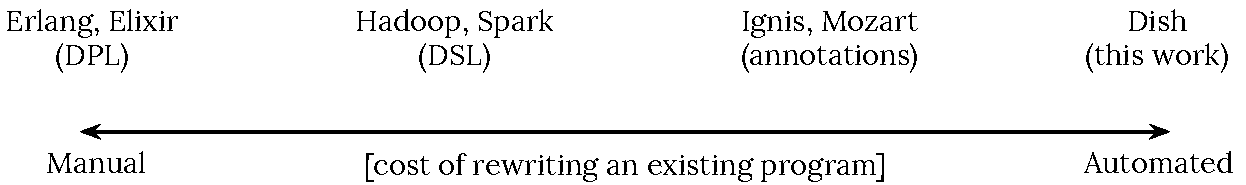
\includegraphics[width=0.49\textwidth]{\detokenize{./figs/dish_spectrum.pdf}}
\caption{
  \textbf{Cost of Manual Effort.}
	\sys sits at the automation end of the spectrum, automatically distributing shell pipelines while maintaining their correctness. A more complete picture is presented in the related-work section~\sx{rt}.
}
\label{fig:spectrum}
\end{figure}

\heading{DSLs for Distribution}
At the other end of the spectrum, distributed computing frameworks~\cite{mapreduce:08, ciel:11, spark:12, naiad:13} and domain-specific languages~\cite{alvaro2011consistency, distal:13, meiklejohn2015lasp, psync:16, dartagnan:18}
simplify certain patterns, 
but do not offer the flexibility of a full-fledged environment.
% suffer from a similar lack of generality by making strong assumptions about the nature of the computation---for example, strongly-eventual commutative components that can proceed in parallel.
Developing under these frameworks differs quite significantly from the development of normal (non-distributed) programs.

More recent work focuses on extracting parallelism from domain-specific programming models~\cite{cilk5, streamIt, galois} and interactive parallelization tools~\cite{parascope, ipat}.
These tools simplify the expression of parallelism, but still require programmers to get involved in discovering and exposing parallelism.
%  actively involve the programmer in the detection and mapping of application parallelism, but still demand great effort from the user. 
Moreover, the insights behind these attempts are significantly different from ours, as they extract parallelism statically during compilation instead of dynamically during runtime.
%Despite significant progress~\cite{}, it remains due to its need for complex program analysis and the unknown factors (such as input data range) during compilation.

\heading{Concurrent and Distributed Shells}
\nv{NV}
Among other work, the Smoosh authors have argued that certain features of the shell are useful for concurrency~\cite{smoosh:18};
Their work does not automatically parallelize pipelines, but rather argues that the shell language is itself an good DSL for concurrency;
This argument is different from \sys, 
an argument complementary to \sys's which automatically (and correcctly) parallelizes pipelines even when developers have---hence distribution-\emph{oblivious} shell scripting.

Several shells add support for non-linear pipe topologies;
  this 
2dsh~\cite{}
rc~\cite{}
gsh~\cite{}
dgsh~\cite{dagsh:17}.

Commands for explicitly specifying parallelism such \ttt{qsub}~\cite{gentzsch2001sun}, \textsc{SLURM}~\cite{yoo2003slurm}, calls to \textsc{GNU} \ttt{parallel}~\cite{Tange2011a}, or any manual rewriting~\cite{mapreduce:08, ciel:11, spark:12}.
These commands require the user to express the program explicitely, work only with embarrasingly parallel (and short) programs;
  \sys and scales out to large pipelines
Often, these commands provide options to support very special cases
---a stark contradiction to the celebrated \unix philosophy.
For example, \tti{parallel}, an official GNU project, flags such as \ttt{--skip-first-line}, \ttt{-trim}, and \ttt{--xargs}, that a \unix user would achieve with \ttt{head}, \ttt{sed}, and \ttt{xargs}; it also includes other programs that 
with complex semantics, such as the ability transfer files between computers, separate text files, and parse CSV.


\heading{Dataflow Graph Model}

\nv{needs KM}
On our dataflow graph model: Our data flow graph model is
  different than most distributed batch and stream processing systems,
  since the shell is a hybrid between the two. Batch processing
  systems have no notion of data order, and stream processing systems
  usually have order, but none of these systems supports this notion
  of reading from different sources in sequence. Our dataflow graph
  model supports this by including information about incoming edge
  order. Another benefit of our dataflow model, is that together with
  the equations that hold on stateless and pure commands, data
  parallelism is exposed in the graph as task parallelism. This allows
  the unoptimized and optimized dataflow graph to have the same
  unified representation, and doesn't lead to an ad-hoc optimization
  of the dataflow graph as done in the other systems (the last bit is
  too aggressive).

\TODO{We have to also cite the paper by Konstantinos, Caleb, Rajeev,
  etc since they also try to do semantics preserving optimizations on
  dataflow graphs}

\km{Some very early references on the dataflow model of computation (maybe there are relevant?): \cite{KM1966, D1974Dataflow, K1974KPN, KMacQ1977}}
  
\cite{HSSGG2014, SHGW2015} discuss optimizing transformations, but their correctness is established using informal arguments based on operational intution.
  
The paper \cite{MSAIT2019} proposes a denotational semantic framework for stream processing where the data streams are seen as partial orders, and establishes the soundness of some common parallelizing transformations on dataflow graphs.


\section{Discussion}
\label{discussion}

This section reflects on \sys's design and implementation, touches on future work, and closes the paper.

\heading{Limitations}
Our is implementation is limited in many ways, so as to succeed in proving the key hypothesis---that scaling out shell pipelines can be automated and correct\TODO{with respect to some assumptions}--- despite \sys being a research prototype.

\sys does not adequately handle failures or network partitions in the general sense, which would include re-scheduling passes that were executing on failed replicas.
Prior work on fault-tolerant distributed stream processing~\cite{} can be of significant aid here.

The logic of the planner is quite simplified, attempting only straightforward placement of tasks to nodes (and using a hard-coded, homogeneous node structure).
Prior work on operator placement of distributed dataflow graphs~\cite{} can be used to improve it.

\sys is conservative in the shell subsets that it handles, in order to
not introduce unsafe behaviours. The point of this work was not to be
able to handle a complete distributable subset of the shell, but
rather use significant part of it to demonstrate performance benefits.

Shell is highly dynamic, thus making it impossible to design sound
meaningful analyses to determine distributable regions and maximal
parallelization. In order to address this particularity, \sys could be
tighly integrated with a posix compliant shell
interpreter~\cite{smoosh:20} so that dynamic information can be
acquired selectively to aid the analysis and optimization process.


\heading{Future Work}
% \label{limitation}
% \item No cycles (multiple commands writing and reading from the same file)
There are several worthwhile directions for future work.  One
direction would be an extension of the distributability analysis of
\sys, in order to guide it using dynamic information. This could
enable a formal study of the analysis~\sx{impl} to show that it
returns regions that are safe to distribute.  Recent work on
formalizing the semantics of the POSIX shell~\cite{smoosh:20} make
such an attempt possible.

Another direction is to extend \sys to handle other classes outside \sta and \pur.
These two classes enjoy a certain in quick, one-off pipelines and are the easiest to distribute, but 
it would be interesting to expand to \dfs (with the use of a distributed file-system) and \sid (with the use of transactional protocols).
This direction would naturally introduce considerations about replication, consistency, and failure recovery.

% There are two additional assumptions that have to be satisfied in
% order for the distributed implementation that is generated by Dish to
% have equivalent behaviour with the original implementation. First of
% all, there should be no external signals to the commands while they
% execute. At the moment Dish assumes no faults, and that communication
% always succeeds. This assumption can be lifted by extending Dish with
% a fault-tolerant runtime, \kk{blah blah}. Second, we assume that no
% command reads and writes to arbitrary files that are not mentioned in
% their arguments. This is a necessary assumption, since commands are
% considered as black boxes and the only information that can be
% inferred about them is through their arguments.

\heading{Conclusion}
This paper presented \sys, a shell variant that automatically and correctly scales out distribution-oblivious shell pipelines. 
\sys's insight is that shell pipelines already express stream computations that can be automatically distributed.
To achieve this, \sys
  decomposes primitives into distributability classes,
  identifies high-distributability stages,
  applies rewriting rules for largest possible subprograms,
  and orchestrates the execution of the distributed program.
% Its runtime component provides orchestration and planning support during the execution of the program.
Experiments with complex pipelines show substantial speedups and the ability to operate on large input datasets, all without any developer input.

\begin{acks}
  % Dumping people so that we don't forget
  % 
  This material is based upon work supported by the
  \grantsponsor{GS100000001}{National Science
    Foundation}{http://dx.doi.org/10.13039/100000001} under Grant
  No.~\grantnum{GS100000001}{nnnnnnn} and Grant
  No.~\grantnum{GS100000001}{mmmmmmm}.  Any opinions, findings, and
  conclusions or recommendations expressed in this material are those
  of the author and do not necessarily reflect the views of the
  National Science Foundation.
\end{acks}


%% Bibliography
\bibliography{./bib}


%% Appendix
\appendix
\section{Scripts used in the evaluation}

This appendix contains the source code of the scripts used in the evaluation of
the \sys. They are part of the codebase (released as open source with the camera
ready), and are provided here only to aid the reviewers.


\end{document}
